%Version 3.1 December 2024
% See section 11 of the User Manual for version history
%
%%%%%%%%%%%%%%%%%%%%%%%%%%%%%%%%%%%%%%%%%%%%%%%%%%%%%%%%%%%%%%%%%%%%%%
%%                                                                 %%
%% Please do not use \input{...} to include other tex files.       %%
%% Submit your LaTeX manuscript as one .tex document.              %%
%%                                                                 %%
%% All additional figures and files should be attached             %%
%% separately and not embedded in the \TeX\ document itself.       %%
%%                                                                 %%
%%%%%%%%%%%%%%%%%%%%%%%%%%%%%%%%%%%%%%%%%%%%%%%%%%%%%%%%%%%%%%%%%%%%%

%%\documentclass[referee,sn-basic]{sn-jnl}% referee option is meant for double line spacing

%%=======================================================%%
%% to print line numbers in the margin use lineno option %%
%%=======================================================%%

%%\documentclass[lineno,pdflatex,sn-basic]{sn-jnl}% Basic Springer Nature Reference Style/Chemistry Reference Style

%%=========================================================================================%%
%% the documentclass is set to pdflatex as default. You can delete it if not appropriate.  %%
%%=========================================================================================%%

%%\documentclass[sn-basic]{sn-jnl}% Basic Springer Nature Reference Style/Chemistry Reference Style

%%Note: the following reference styles support Namedate and Numbered referencing. By default the style follows the most common style. To switch between the options you can add or remove “Numbered” in the optional parenthesis. 
%%The option is available for: sn-basic.bst, sn-chicago.bst%  
 
%%\documentclass[pdflatex,sn-nature]{sn-jnl}% Style for submissions to Nature Portfolio journals
%%\documentclass[pdflatex,sn-basic]{sn-jnl}% Basic Springer Nature Reference Style/Chemistry Reference Style
\documentclass[pdflatex,sn-mathphys-num]{sn-jnl}% Math and Physical Sciences Numbered Reference Style
%%\documentclass[pdflatex,sn-mathphys-ay]{sn-jnl}% Math and Physical Sciences Author Year Reference Style
%%\documentclass[pdflatex,sn-aps]{sn-jnl}% American Physical Society (APS) Reference Style
%%\documentclass[pdflatex,sn-vancouver-num]{sn-jnl}% Vancouver Numbered Reference Style
%%\documentclass[pdflatex,sn-vancouver-ay]{sn-jnl}% Vancouver Author Year Reference Style
%%\documentclass[pdflatex,sn-apa]{sn-jnl}% APA Reference Style
%%\documentclass[pdflatex,sn-chicago]{sn-jnl}% Chicago-based Humanities Reference Style

%%%% Standard Packages
%%<additional latex packages if required can be included here>

\usepackage{graphicx}%
\usepackage{multirow}%
\usepackage{amsmath,amssymb,amsfonts}%
\usepackage{amsthm}%
\usepackage{mathrsfs}%
\usepackage[title]{appendix}%
\usepackage{xcolor}%
\usepackage{textcomp}%
\usepackage{manyfoot}%
\usepackage{booktabs}%
\usepackage{algorithm}%
\usepackage{algorithmicx}%
\usepackage{algpseudocode}%
\usepackage{listings}%

\usepackage{kotex}
%%%%

%%%%%=============================================================================%%%%
%%%%  Remarks: This template is provided to aid authors with the preparation
%%%%  of original research articles intended for submission to journals published 
%%%%  by Springer Nature. The guidance has been prepared in partnership with 
%%%%  production teams to conform to Springer Nature technical requirements. 
%%%%  Editorial and presentation requirements differ among journal portfolios and 
%%%%  research disciplines. You may find sections in this template are irrelevant 
%%%%  to your work and are empowered to omit any such section if allowed by the 
%%%%  journal you intend to submit to. The submission guidelines and policies 
%%%%  of the journal take precedence. A detailed User Manual is available in the 
%%%%  template package for technical guidance.
%%%%%=============================================================================%%%%

%% as per the requirement new theorem styles can be included as shown below
\theoremstyle{thmstyleone}%
\newtheorem{theorem}{Theorem}%  meant for continuous numbers
%%\newtheorem{theorem}{Theorem}[section]% meant for sectionwise numbers
%% optional argument [theorem] produces theorem numbering sequence instead of independent numbers for Proposition
\newtheorem{proposition}[theorem]{Proposition}% 
%%\newtheorem{proposition}{Proposition}% to get separate numbers for theorem and proposition etc.

\theoremstyle{thmstyletwo}%
\newtheorem{example}{Example}%
\newtheorem{remark}{Remark}%

\theoremstyle{thmstylethree}%
\newtheorem{definition}{Definition}%

\raggedbottom
%%\unnumbered% uncomment this for unnumbered level heads

\begin{document}

\title[Article Title]{Live Mobile Learning System with User-Adjustable UI}

%%=============================================================%%
%% GivenName	-> \fnm{Joergen W.}
%% Particle	-> \spfx{van der} -> surname prefix
%% FamilyName	-> \sur{Ploeg}
%% Suffix	-> \sfx{IV}
%% \author*[1,2]{\fnm{Joergen W.} \spfx{van der} \sur{Ploeg} 
%%  \sfx{IV}}\email{iauthor@gmail.com}
%%=============================================================%%

\author{\fnm{Hosung} \sur{Kim}}\email{hosungkim5108@gmail.com}

%%\author[2,3]{\fnm{Second} \sur{Author}}\email{iiauthor@gmail.com}
%%\equalcont{These authors contributed equally to this work.}

%%\author[1,2]{\fnm{Third} \sur{Author}}\email{iiiauthor@gmail.com}
%%\equalcont{These authors contributed equally to this work.}

\affil{\orgdiv{Department of Computer Engineering}, \orgname{Hongik University}, \orgaddress{ \city{Seoul}, \country{Korea}}}

\abstract{기존 원격 교육 시스템은 대부분 강의자료와 화이트보드를 함께 배치하지 않아, 강의자료와 칠판을 함께 볼 수 있는 실제 강의 환경과 차이가 있다. 두 콘텐츠를 함께 배치하더라도 모바일 기기의 제한된 화면 크기로 인해 정보가 지나치게 축소되면 강의자의 활용과 학습자의 이해에 제약이 따른다. 본 보고서에서는, 강의자가 두 콘텐츠 영역의 크기를 자유롭게 조절할 수 있는 User-Adjustable UI 기반의 모바일 원격 교육 시스템을 설계하고 구현하였다. 이를 통해 학습자는 제한된 크기의 화면에서도 정보를 충분한 크기로 확인할 수 있어 실제 강의와 유사한 경험을 제공한다. 사용자 만족도 조사 결과, 제시된 시스템은 기존 시스템보다 높은 평가를 받아, User-Adjustable UI가 모바일 원격 교육 환경에서 학습 효과를 향상시킴을 확인하였다.}

%%\keywords{keyword1, Keyword2, Keyword3, Keyword4}

%%\pacs[JEL Classification]{D8, H51}

%%\pacs[MSC Classification]{35A01, 65L10, 65L12, 65L20, 65L70}

\maketitle

\section{Introduction}\label{sec1}

COVID-19 팬데믹으로 인해 전 세계적으로 대면 수업이 제한되면서 교육 현장은 급격한 변화를 맞이하였다. 이 과정에서 온라인 기반의 원격 교육이 대면 수업을 대체하는 핵심 수단으로 부상하였으며, 특히 모바일 기기를 활용한 원격 교육은 학습의 공간적 제약을 해소하고 접근성을 높였다. 결과적으로 모바일 원격 교육은 팬데믹 상황에서의 일시적인 대책을 넘어 새로운 교육 패러다임으로 자리매김하였다.

팬데믹 기간 동안 교육 현장에는 Cisco Webex\cite{Webex}, Zoom\cite{Zoom}, Microsoft Teams\cite{MicrosoftTeams}, Google Meet\cite{GoogleMeet}와 같은 화상회의 기반의 원격 교육 플랫폼이 널리 활용되었다. 이러한 플랫폼들은 강의자료 공유, 채팅, 강사의 음성 및 영상 송출, 강의자료에 대한 실시간 주석 작성, 화이트보드, 참여자 명단 등 다양한 기능을 제공하여 비대면 환경에서도 원활한 수업 진행과 상호작용이 가능하도록 지원하였다.

그러나 기존 모바일 원격 교육 시스템들은 강의자료와 화이트보드를 함께 배치하지 않아, 강의자료와 칠판을 동시에 볼 수 있는 실제 강의 환경과 유사한 경험을 제공하지 못한다. 이러한 한계는 대면 강의를 온전히 대체하는 데 제약이 된다. 이를 보완하기 위해 두 콘텐츠를 한 화면에 병렬로 배치하는 방식이 고려될 수 있으나, 제한된 크기의 화면에서 정보가 지나치게 축소되면 오히려 강의자의 활용과 학습자의 이해에 부정적인 영향을 미칠 수 있다.

따라서 본 보고서에서는 강의자료와 화이트보드를 함께 배치하면서도 제한된 크기의 화면 공간을 효율적으로 활용할 수 있는 User-Adjustable UI 기반의 모바일 원격 교육 시스템을 설계 및 구현하였다. 제시된 시스템에 적용된 User-Adjustable UI는 grabber를 통해 두 콘텐츠 영역의 크기를 자유롭게 조절할 수 있어서 강의 상황에 맞추어 필요한 정보를 유연하게 강조할 수 있다. 또한 제시된 시스템은 강의자료 공유, 채팅, 강사의 음성 및 영상 송출, 강의자료에 대한 실시간 주석 작성, 화이트보드, 참여자 명단 등 기존 원격 교육 시스템의 핵심 기능을 모두 포함하고 있다.

\section{Design}\label{sec2}

그림\ref{fig1}은 제시된 시스템의 통신 아키텍쳐를 보여준다. 제시된 시스템은 강사측 모바일 클라이언트, 학생측 모바일 클라이언트, 서버로 이루어져있다.

\begin{figure}[H]
\centering
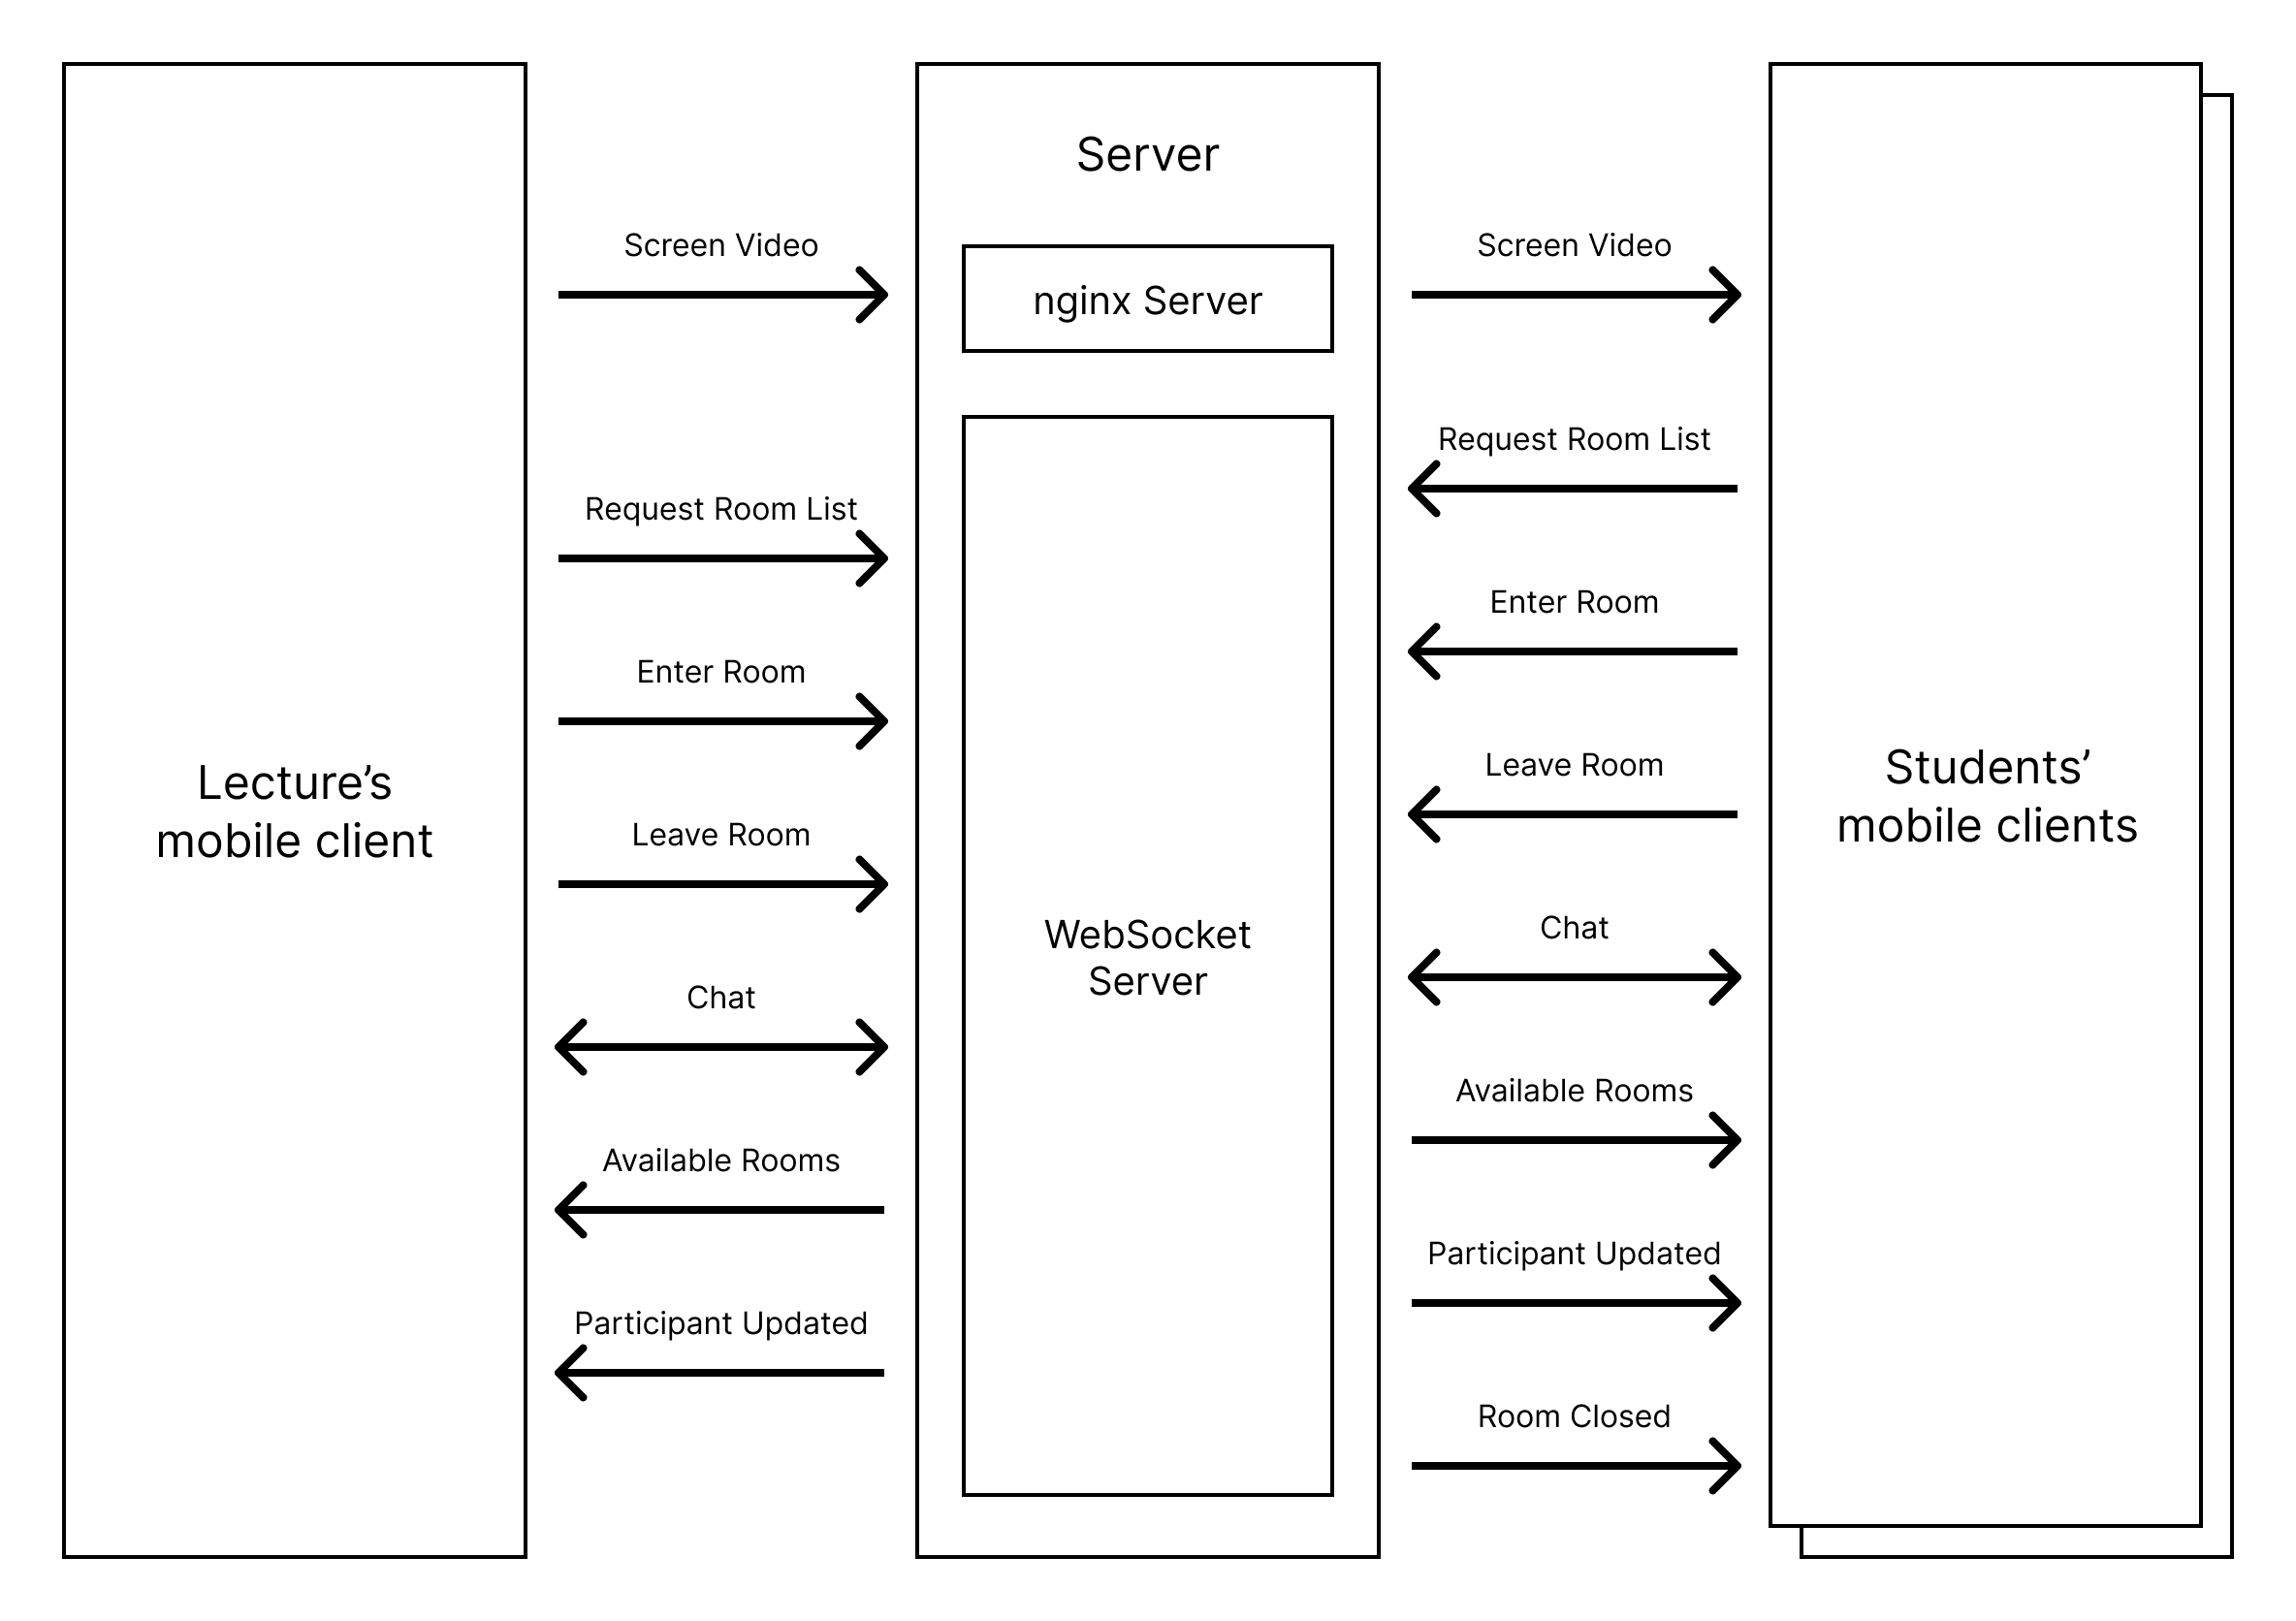
\includegraphics[width=0.9\textwidth]{communication_architecture.png}
\caption{Communication architecture of the proposed system}\label{fig1}
\end{figure}

\subsection{Server}\label{subsec1}

서버는 NGINX\cite{NGINX} 기반의 스트리밍 서버와 WebSocket 서버로 이루어져있다. 강사측 모바일 클라이언트는 음성과 영상을 실시간으로 스트리밍 서버에 전송하고, 학생측 모바일 클라이언트는 스트리밍 서버로부터 데이터를 수신한다. WebSocket 서버는 강의실 생성, 입장 및 퇴장, 강의실 종료, 강의실 목록 조회, 참여자 명단 동기화 등 다중 강의실 기능과 채팅 기능을 제공한다.

\subsection{Client}\label{subsec2} 

클라이언트 애플리케이션은 Clean Architecture\cite{martin2017clean}와 MVVM(Model - View - ViewModel) 아키텍쳐 패턴을 결합하여 설계되었다. Clean Architecture는 애플리케이션을 계층화하여 각 계층의 책임을 명확하게 함으로써, 재사용성과 테스트 용이성을 높이는 데 목적이 있다. 본 애플리케이션은 그림\ref{fig2}에서 볼 수 있듯이 Data, Domain, Presentation 세 계층으로 구성되고 각 계층에 대한 자세한 설명은 다음과 같다.

Data 계층은 Service, DTO, Repository(Implementation)로 구성되며, 서버와의 직접적인 통신을 담당한다. Domain 계층은 Entity, Repository(Protocol), UseCase로 구성되며, 핵심 데이터와 비즈니스 로직을 포함한다. Presentation 계층은 ViewModel, ViewController로 구성되고, UI를 통해 User와 직접 소통한다.

서버와 클라이언트 간의 데이터 흐름은 다음과 같다.
서버로부터 데이터를 수신하는 경우, Service가 서버로부터 DTO 형태의 데이터를 전달받고 Repository에서 Entity로 변환한다. 이후 UseCase를 거쳐 ViewModel에 전달된다. ViewController는 ViewModel의 상태 변화를 관찰하고 있다가 변경사항이 발생하면 이를 UI에 반영한다.
서버로 데이터를 전송하는 경우, ViewController에서 ViewModel, UseCase, Repository를 통해 값을 전달한다. Repository를 거치며 Entity는 DTO형태로 변환되고 최종적으로 Service를 통해 서버로 전송한다.

\begin{figure}[H]
\centering
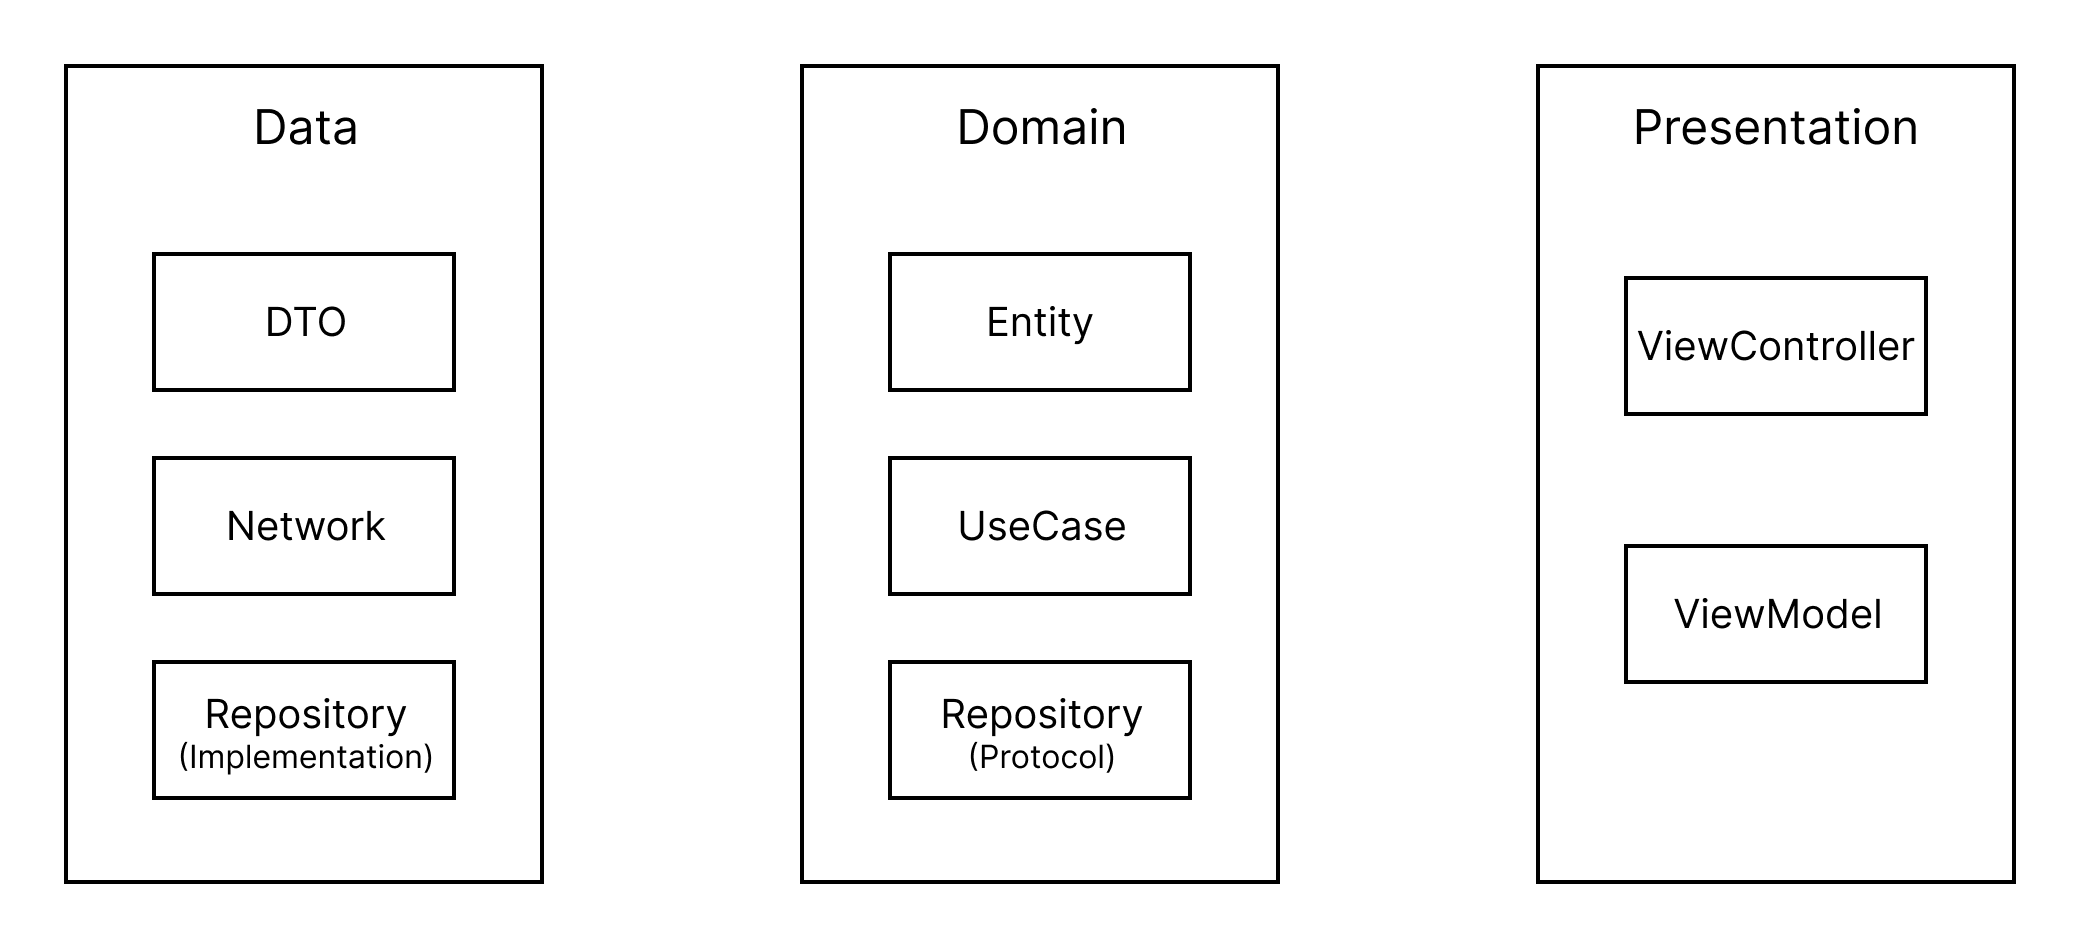
\includegraphics[width=0.9\textwidth]{architecture_of_client.png}
\caption{Architecture of a client}\label{fig2}
\end{figure}

\section{Implementation}\label{sec3}

\subsection{Server}\label{subsec3}

제시된 시스템의 서버는 NGINX 기반의 RTMP(Real-Time Messaging Protocol)\cite{RTMP} 스트리밍 서버와 Swift Network Framework를 이용하여 구현한 WebSocket 서버로 구성된다. 두 서버는 macOS 환경에서 Xcode Command Line Tool로 통합되어 하나의 Xcode Target으로 실행된다.

스트리밍 서버는 서버 실행 시 \verb+Process()+를 통해 nginx.exe 실행파일과 nginx.conf 설정파일을 프로그램적으로 호출하여 자동으로 실행되며, 종료 시에도 동일한 방식으로 제어된다. 이를 통해 운영자는 별도의 명령 입력 없이 안정적으로 서버를 일원화하여 관리할 수 있다.

WebSocket 서버는 Swift Network Framework\cite{Network}의 \verb+NWProtocolWebSocket+을 기반으로 구현되었으며, 강의실 생성·종료·입장·퇴장, 강의실 목록 조회, 참여자 명단 동기화 등 다중 강의실 기능과 채팅 기능을 제공한다. 이처럼 다양한 기능을 제공하기 위해 서버-클라이언트 간 통신에는 \verb+Codable+을 상속한 \verb+enum+을 사용하여 기능 확장을 용이하게 하고 다양한 종류의 메세지를 주고받을 수 있도록 하였다.

WebSocket 서버는 모든 강의실을 UUID를 키로 하는 딕셔너리 형태로 관리한다. 강의실 목록이 변경되면 Available Room 메세지를 모든 클라이언트에게 브로드캐스트한다. Enter Room 또는 Leave Room 메세지를 수신하면 해당 클라이언트를 관련 강의실에 등록하거나 제거한다. 강의자가 퇴장하면 해당 강의실의 모든 학생에게 Room Closed 메세지를 전송하여 강의 종료를 알린다. 참여자 명단 변경이나 채팅 메세지 수신 시, 해당 강의실의 모든 클라이언트에게 각각 Participant Updated 메세지 또는 채팅 메세지를 동일 강의실 내 모든 클라이언트에게 브로드캐스트한다.

\subsection{Client}\label{subsec4}

그림\ref{fig3}은 홈화면을 보여준다. 홈화면에서는 강의실 목록들 중 하나를 선택하여 학생으로 입장하거나 우측 하단의 +버튼을 눌러 강의실을 새로 생성하여 강사로 수업을 시작할 수 있다. 강의실 목록은 WebSocket 서버와의 통신을 통해 실시간으로 갱신되며, 강의실 명단 \verb+UITableView+를 아래로 스크롤하여 수동으로 새로고침할 수도 있다. 강의실 입장과 생성 이벤트는 Enter Room 메세지를 WebSocket 서버에 전송하여 처리된다.

\begin{figure}[H]
\centering
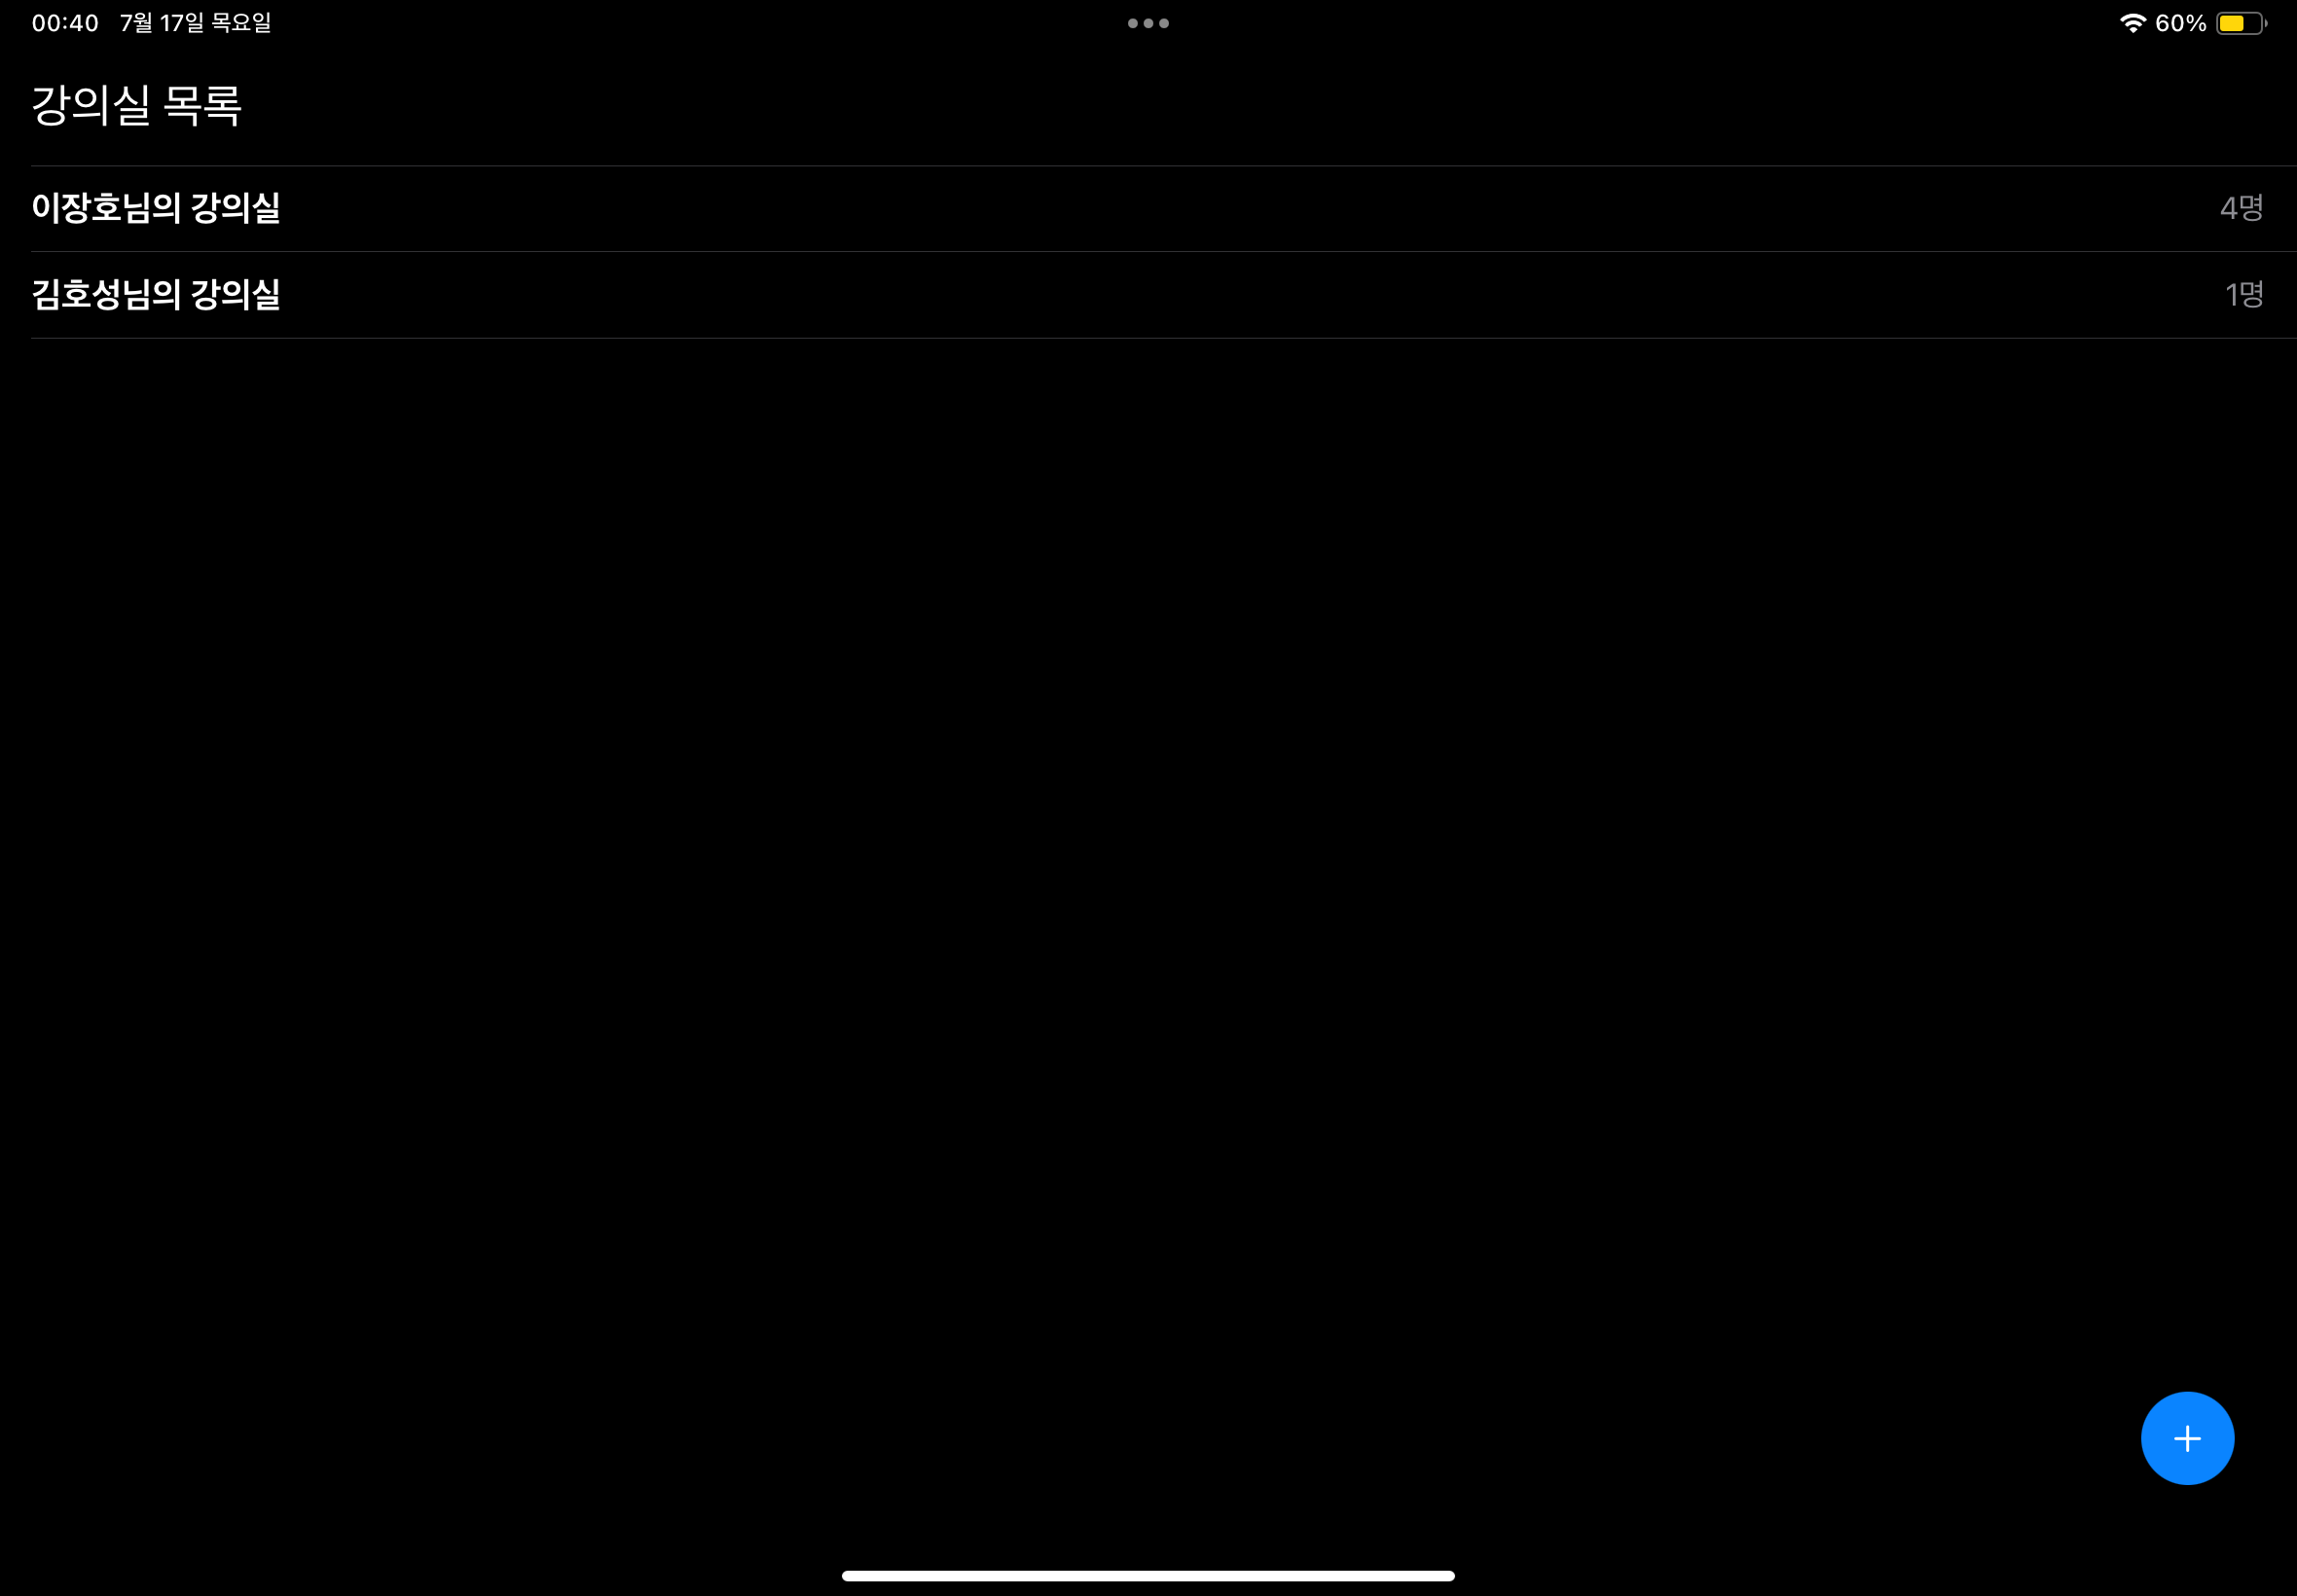
\includegraphics[width=0.9\textwidth]{home.PNG}
\caption{User interface of a home screen}\label{fig3}
\end{figure}

\noindent
그림\ref{fig4}는 강사측 클라이언트의 강의실화면을 보여준다. 해당 화면의 UI는 PDF 강의자료, 화이트보드, 강사 카메라 영상, 참여자 명단, 채팅창 등으로 구성된다. 각 요소에 대한 자세한 설명은 다음과 같다.

\begin{figure}[H]
\centering
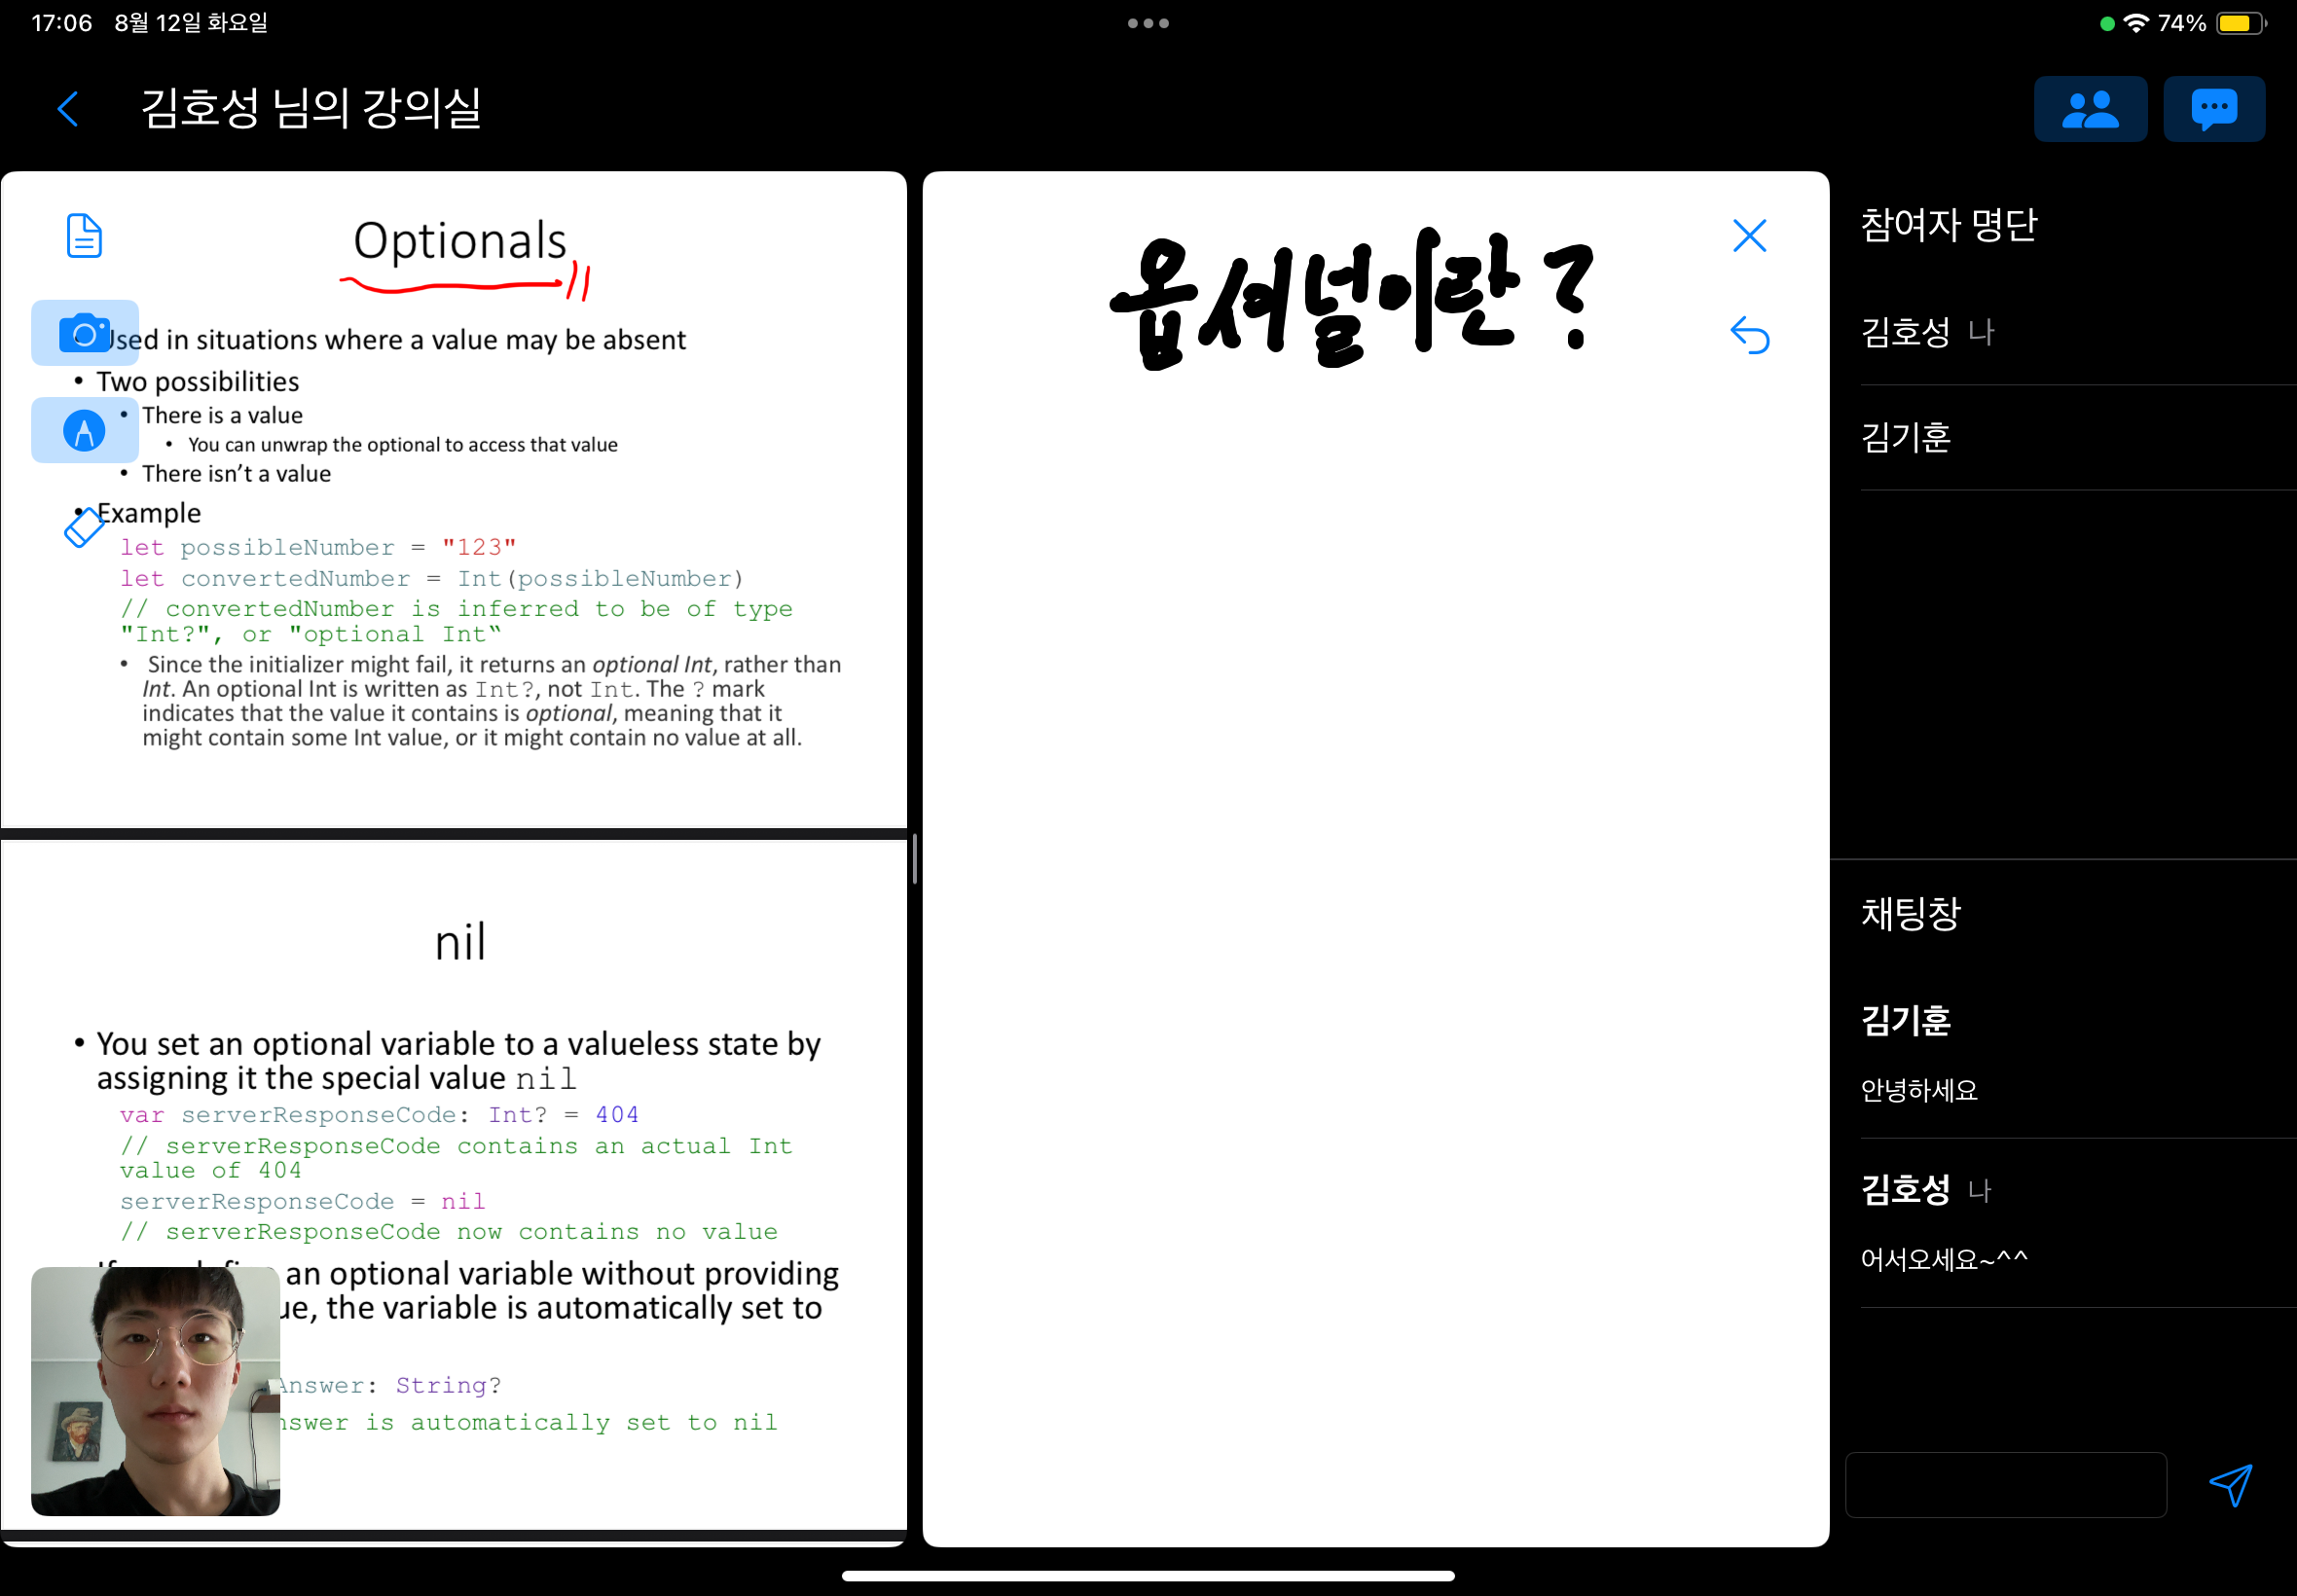
\includegraphics[width=0.9\textwidth]{room0.PNG}
\caption{User interface of a classroom screen}\label{fig4}
\end{figure}

\noindent
PDF 강의자료는 Apple Framework인 PDFKit\cite{PDFKit}의 \verb+PDFView+를 사용하여 구현되었다. 좌측 상단 문서 모양 버튼을 누르면 \verb+UIDocumentPickerViewController+를 통해 기기에 저장된 PDF 파일을 선택할 수 있고 선택된 파일의 링크를 가져와서 \verb+PDFView+로 화면에 출력한다.

강의자료의 주석 기능은 PDFKit의 \verb+PDFPageOverlayViewProvider+를 사용하여 각 \verb+PDFPage+의 \verb+overlayView+에 PencilKit\cite{PencilKit}의 \verb+PKCanvasView+를 추가하여 구현하였다. 좌측 상단의 펜 버튼과 지우개 버튼은 토글식으로 구현되어서 선택되어있는 버튼에 따라 \verb+PKTool+을 펜 또는 지우개로 설정한다. 둘 다 비활성화된 상태일 때는 PDF 문서 스크롤로 작동한다.

화이트보드는 사용자의 터치 이벤트를 직접 감지하여 선을 그리는 방식으로 구현하였다. 터치 이벤트를 \verb+override+하여 사용자가 화면을 터치하면 \verb+touchesBegan+에서 새로운 \verb+UIBezierPath+ 객체를 생성하고 배열에 저장하며, 터치 이동 시에는 \verb+touchesMoved+에서 해당 객체에 좌표를 추가하고 \verb+setNeedsDisplay()+를 호출하여 화면을 갱신하였다. 저장된 \verb+UIBezierPath+들은 \verb+override+한 \verb+draw+ 함수에서 그려진다. 우측 상단 버튼들을 통해 undo와 clear 기능도 지원한다.

강사의 전면 카메라의 영상은 \verb+AVCaptureVideoPreviewLayer+를 기반으로 구현한 \verb+CameraPreviewView+를 통해 제공된다. \verb+CameraPreviewView+는 \verb+UIView+를 상속하며, \verb+layerClass+를 \verb+AVCaptureVideoPreviewLayer+로 지정하여 \verb+AVCaptureSession+을 통해 전면 카메라 영상을 실시간으로 렌더링하여 강의자가 자신의 영상 상태를 직접 확인할 수 있도록 하였다.

그림\ref{fig4}, \ref{fig5}, \ref{fig6}과 같이 참여자 목록과 채팅창은 접이식 구조로 구현하여 불필요한 화면 점유를 최소화하였다. 두 구성요소는 \verb+UIStackView+에 포함되어 있으며, 우측 상단 각각의 토글 버튼에 따라 \verb+isHidden+ 속성을 조정함으로써 열고 닫을 수 있도록 구현하였다.

\begin{figure}[H]
\centering
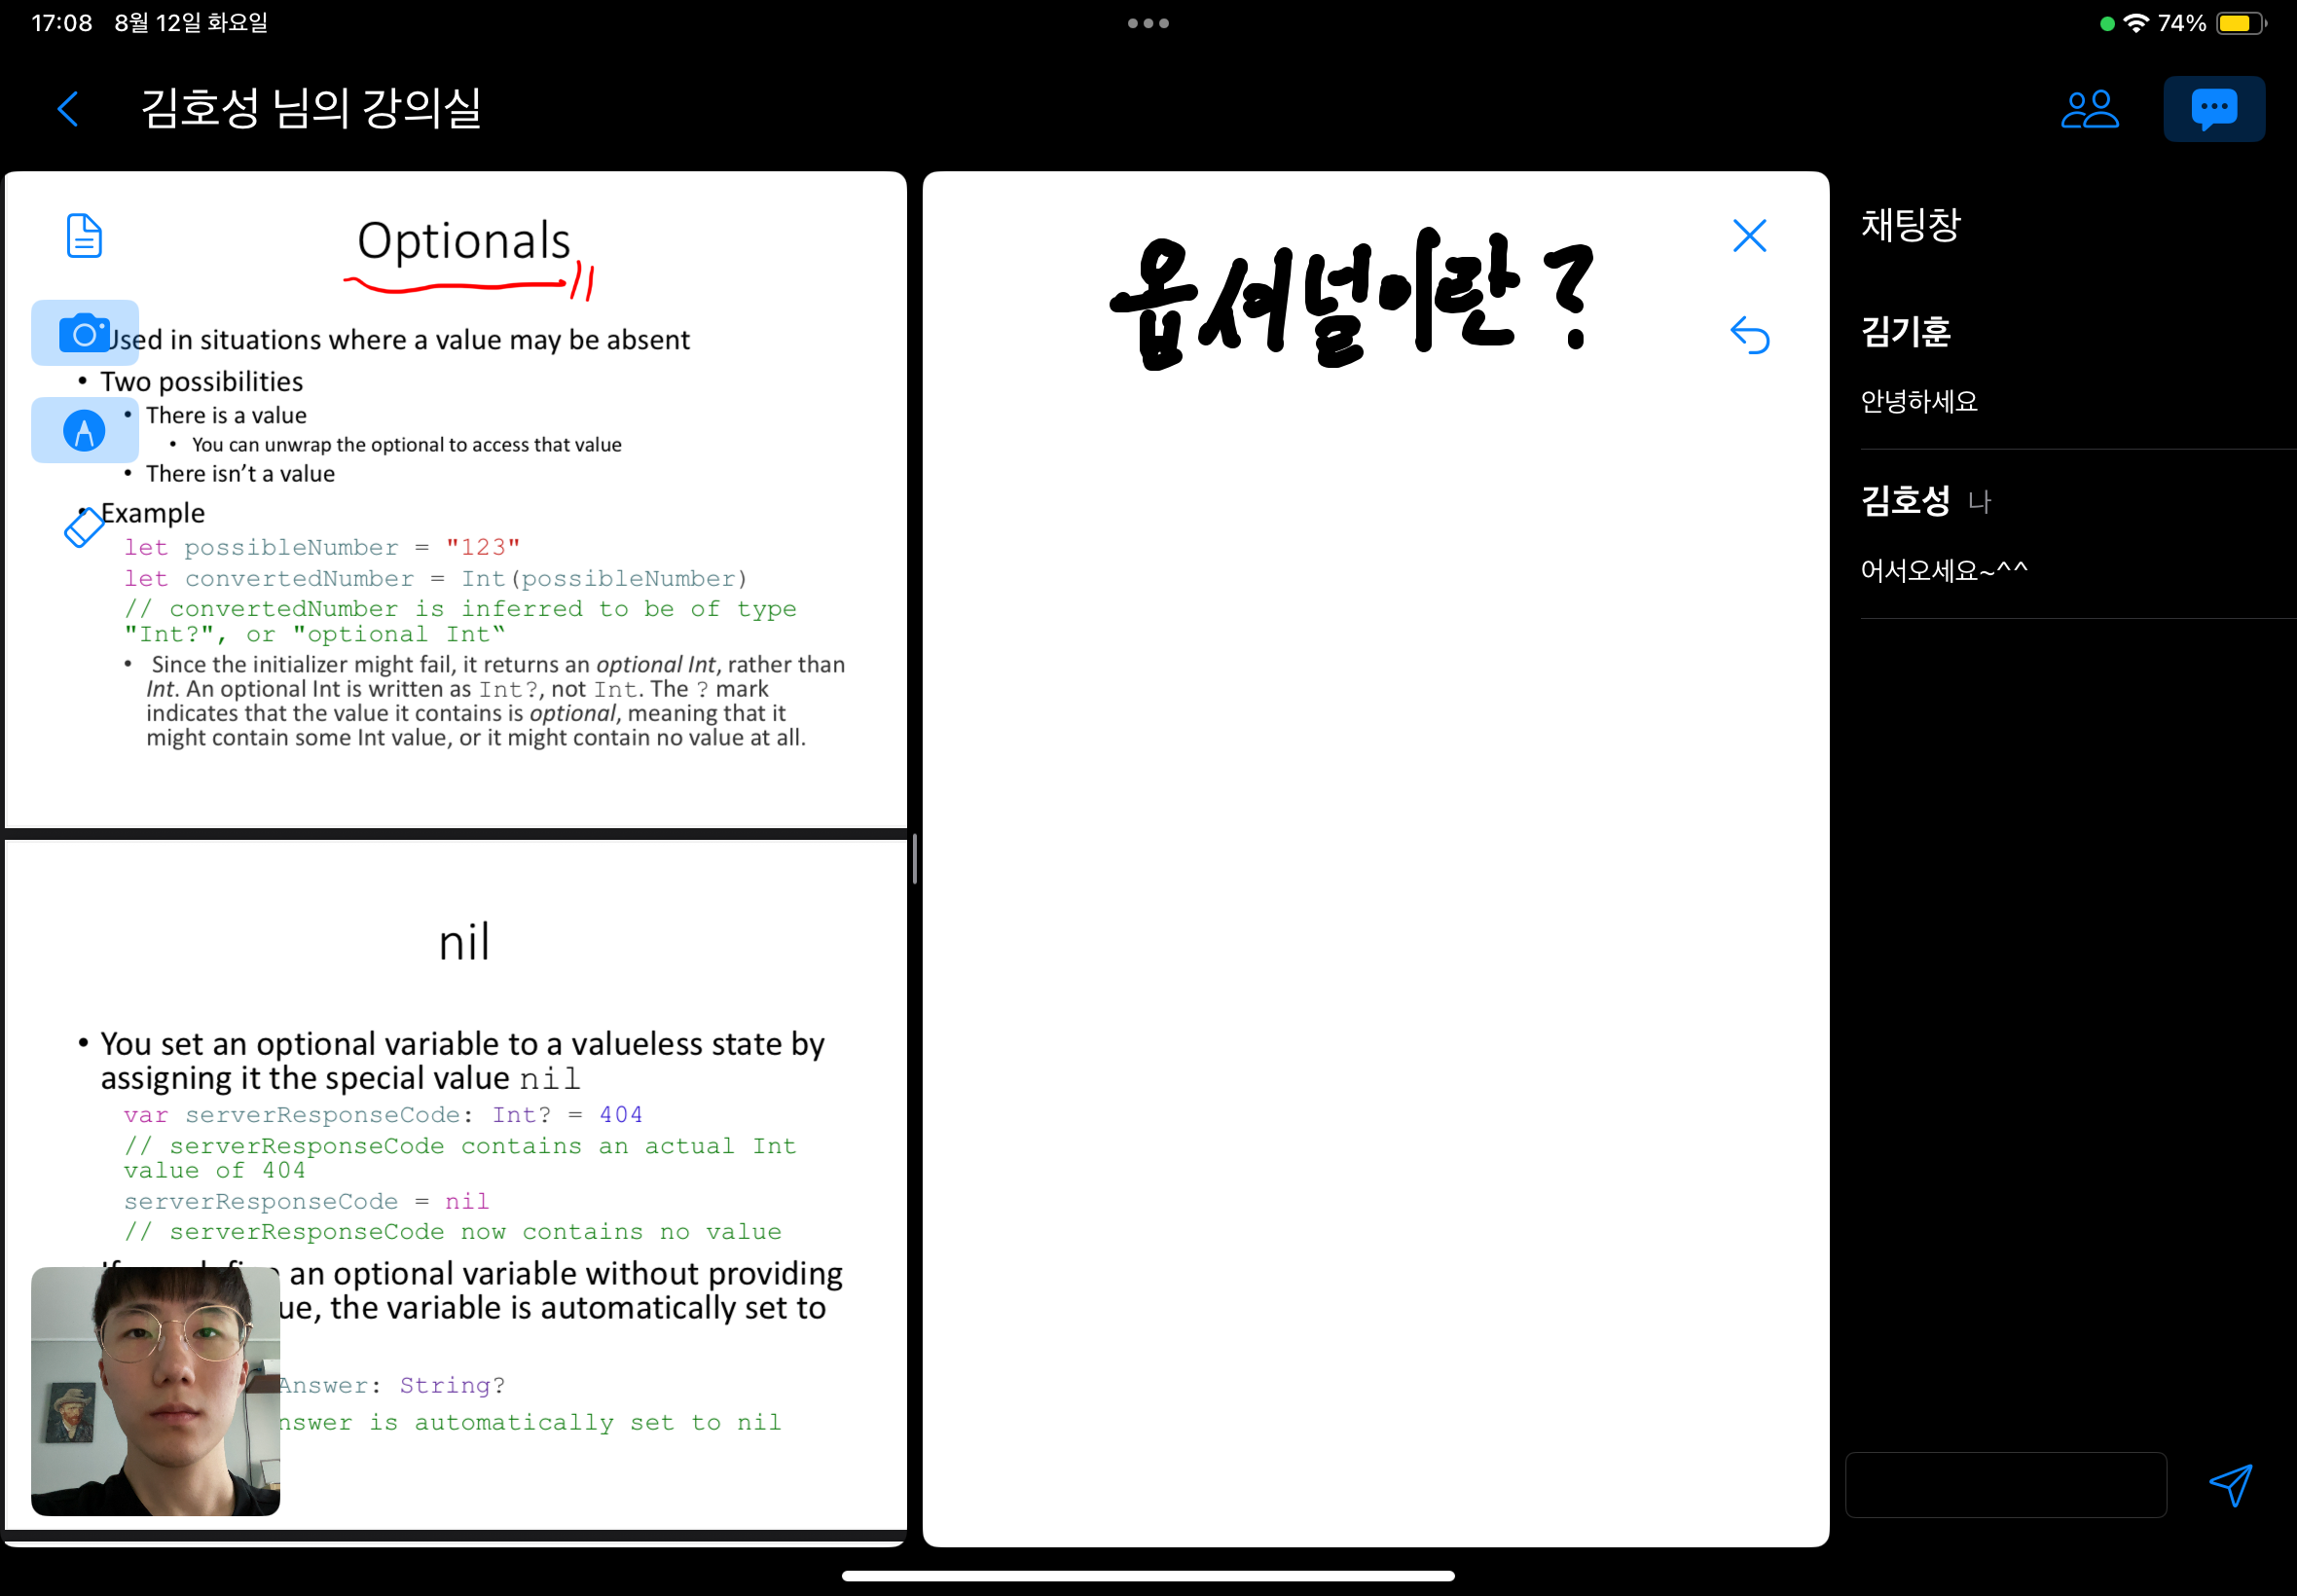
\includegraphics[width=0.9\textwidth]{room1.PNG}
\caption{User interface of a classroom screen with participants panel hidden}\label{fig5}
\end{figure}

\begin{figure}[H]
\centering
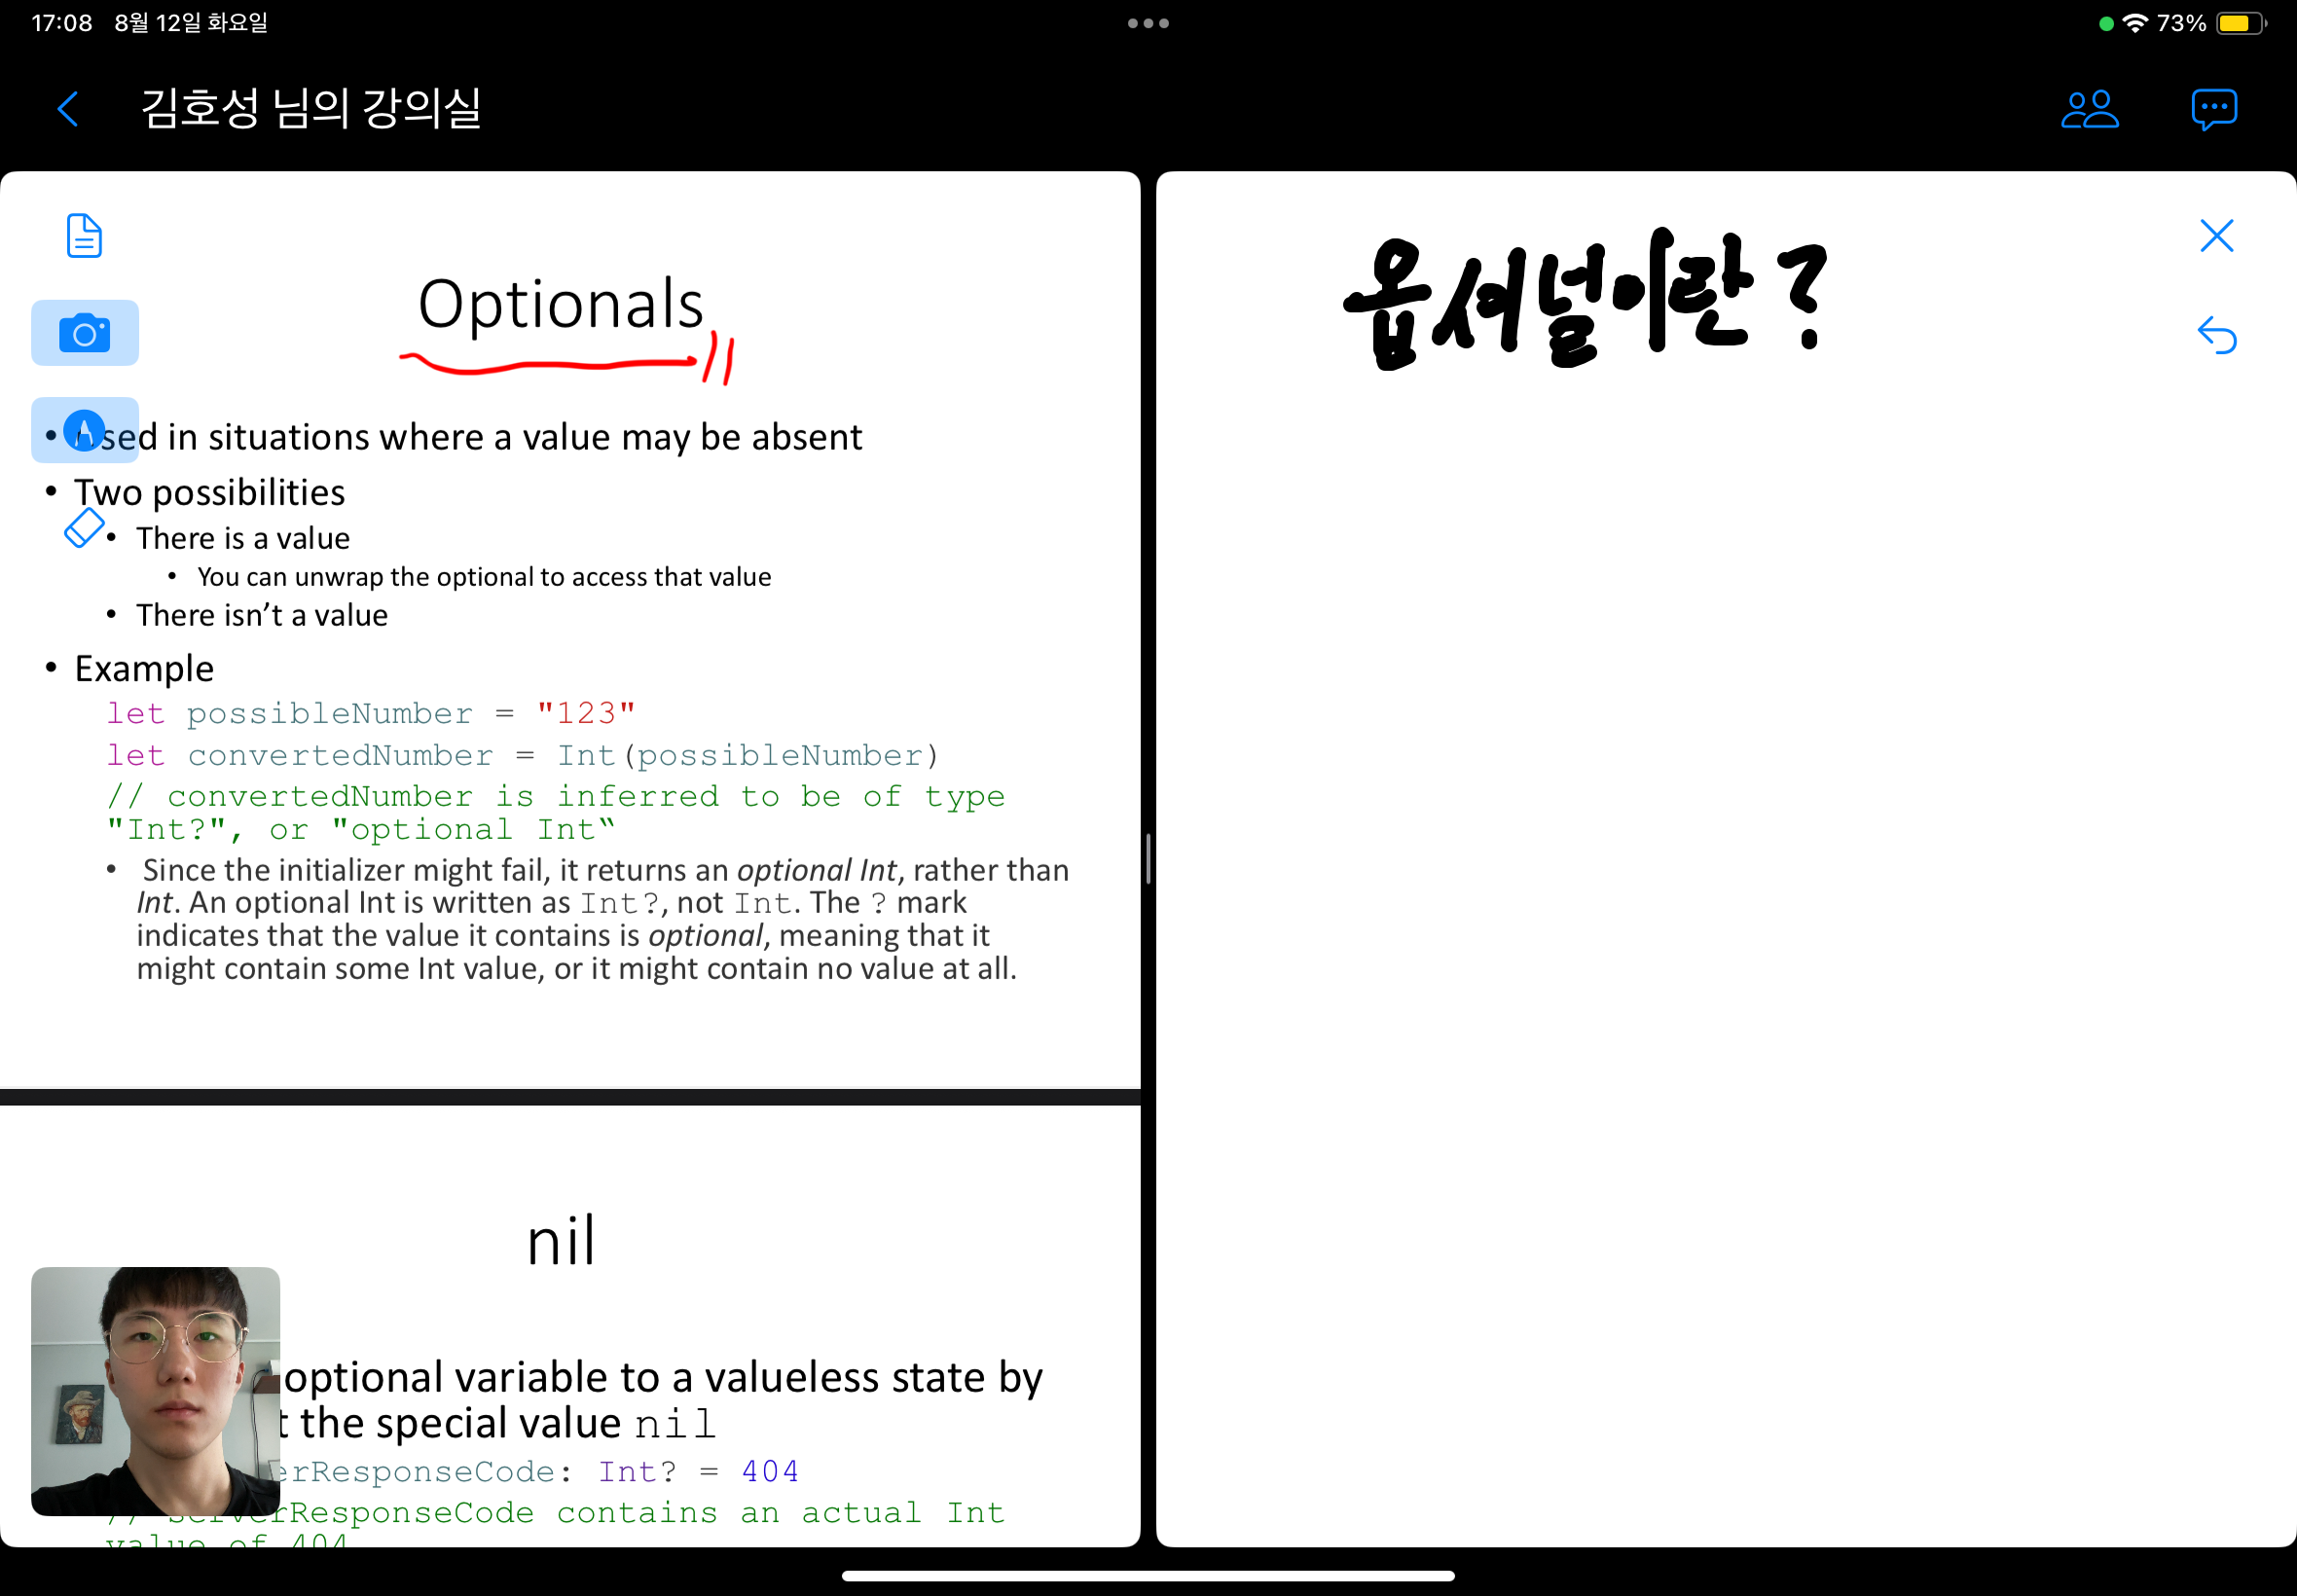
\includegraphics[width=0.9\textwidth]{room2.PNG}
\caption{User interface of a classroom screen with participants and chat panels hidden}\label{fig6}
\end{figure}

\noindent
화면 녹화는 Apple Framework인 ReplayKit\cite{ReplayKit}을 사용하였다. ReplayKit은 전체 화면의 녹화 영상만을 제공하지만, 불필요한 UI의 전송을 방지하고 핵심 콘텐츠만 송출하기 위해 녹화 영상에서 강의자료와 화이트보드 영역만을 잘라내어 사용하였다. 음성은 AVAudioEngine을 통해 AVAudioBuffer 형태로 가져왔다.

이렇게 가져온 영상과 음성은 \verb+StreamService+의 \verb+MediaMixer+에서 하나의 스트림으로 합성된다. 합성된 스트림의 송출은 HaishinKit.swift\cite{HaishinKit} 라이브러리를 기반으로 스트리밍 서버와 직접 RTMP 통신을 수행하는 RTMPService에 의해 이루어진다. RTMPService는 RTMPConnection을 통해 스트리밍 서버와의 연결을 수립하고, RTMPStream을 통해 송출과 수신을 한다. 이때, 서버에서 강의실 생성 시 부여한 UUID 기반의 고유한 키 값을 streamName으로 설정하여 알맞은 강의실에 연결해 송출과 수신을 수행한다.

위 과정을 통해 RTMPService를 통해 강사의 화면과 음성은 실시간으로 송출되고, 학생들은 해당 강의실의 스트림을 수신할 수 있다. 이로써 강의자료와 화이트보드 두 핵심 콘텐츠를 학생에게 동시에 제공할 수 있는 기술적 기반이 마련되었다. 그러나 모바일 기기의 제한된 크기의 화면에서 두 핵심 콘텐츠가 과도하게 작아지지 않도록 하는 UI 설계가 필요하였다.

따라서 강의자가 상황에 맞게 두 콘텐츠 영역의 크기를 조절할 수 있는 User-Adjustable UI를 적용하였다. 그림\ref{fig7}, \ref{fig8}과 같이 강의자는 grabber를 드래그하여 강의자료와 화이트보드의 화면 비율을 자유롭게 조절하며 강의 상황에 따라 필요한 정보를 유연하게 강조할 수 있다.

\begin{figure}[H]
\centering
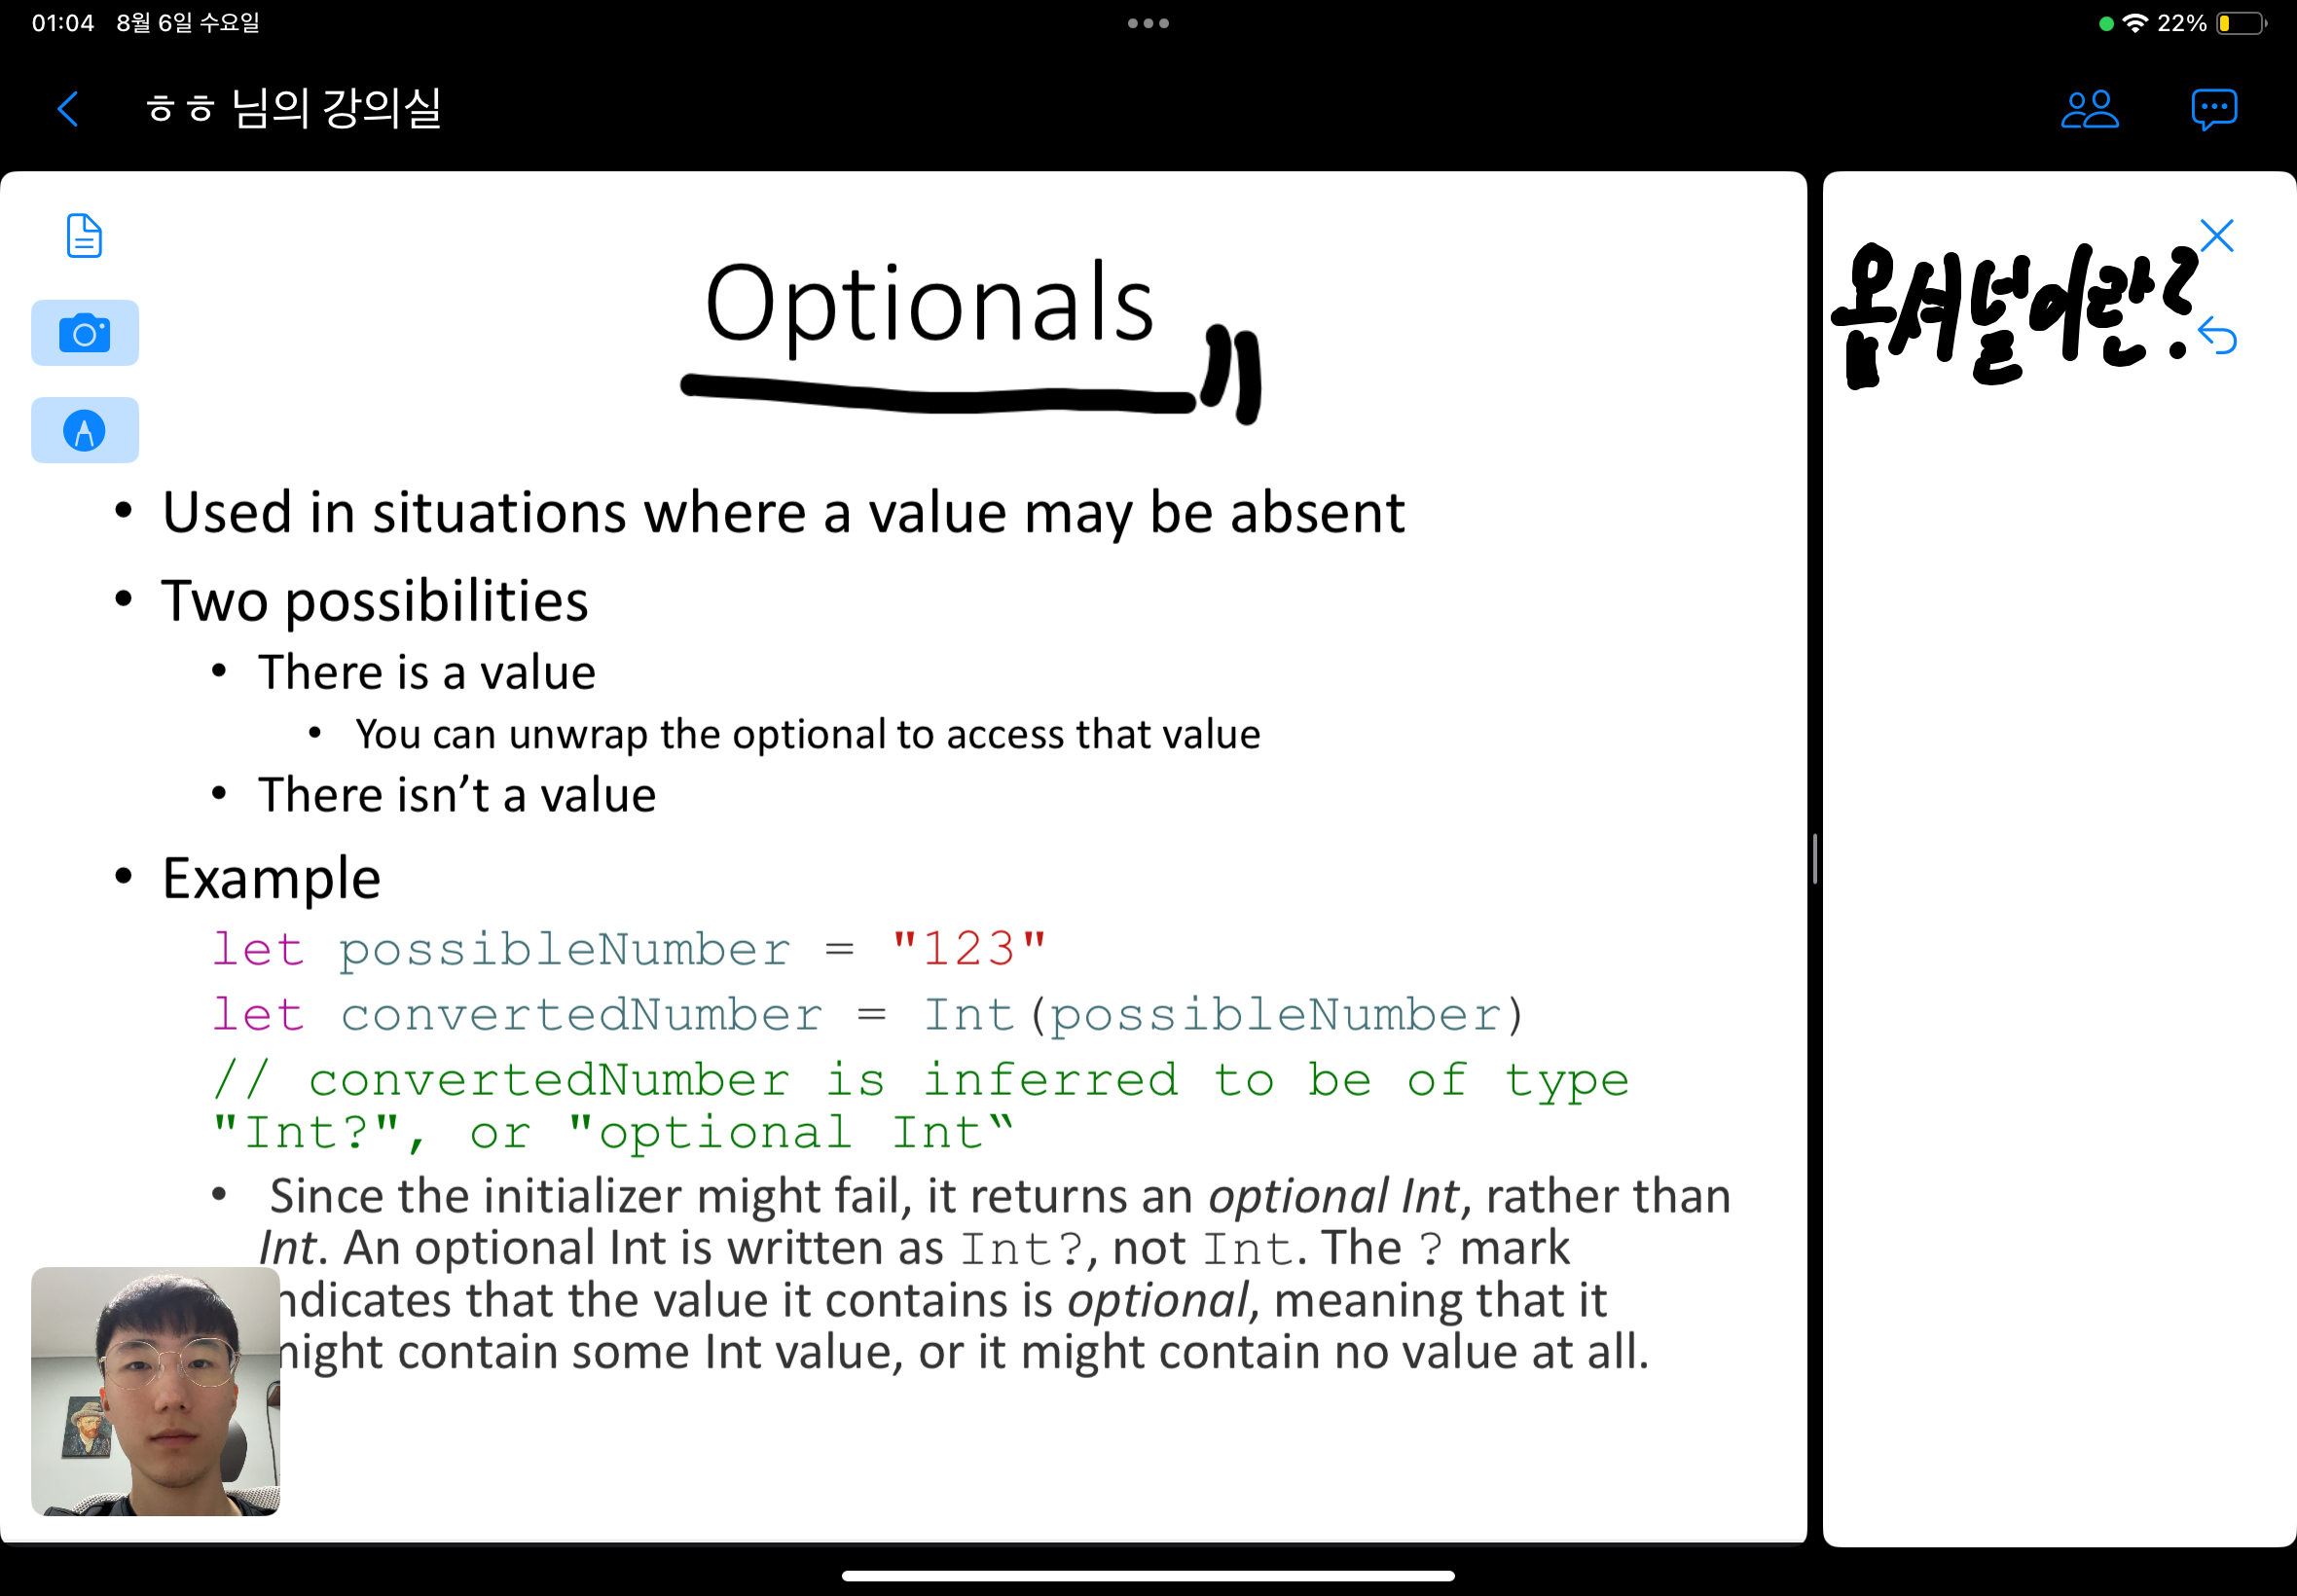
\includegraphics[width=0.9\textwidth]{UserInterfaceWithAnExpandedDocumentArea.PNG}
\caption{User interface with an expanded document area}\label{fig7}
\end{figure}

\begin{figure}[H]
\centering
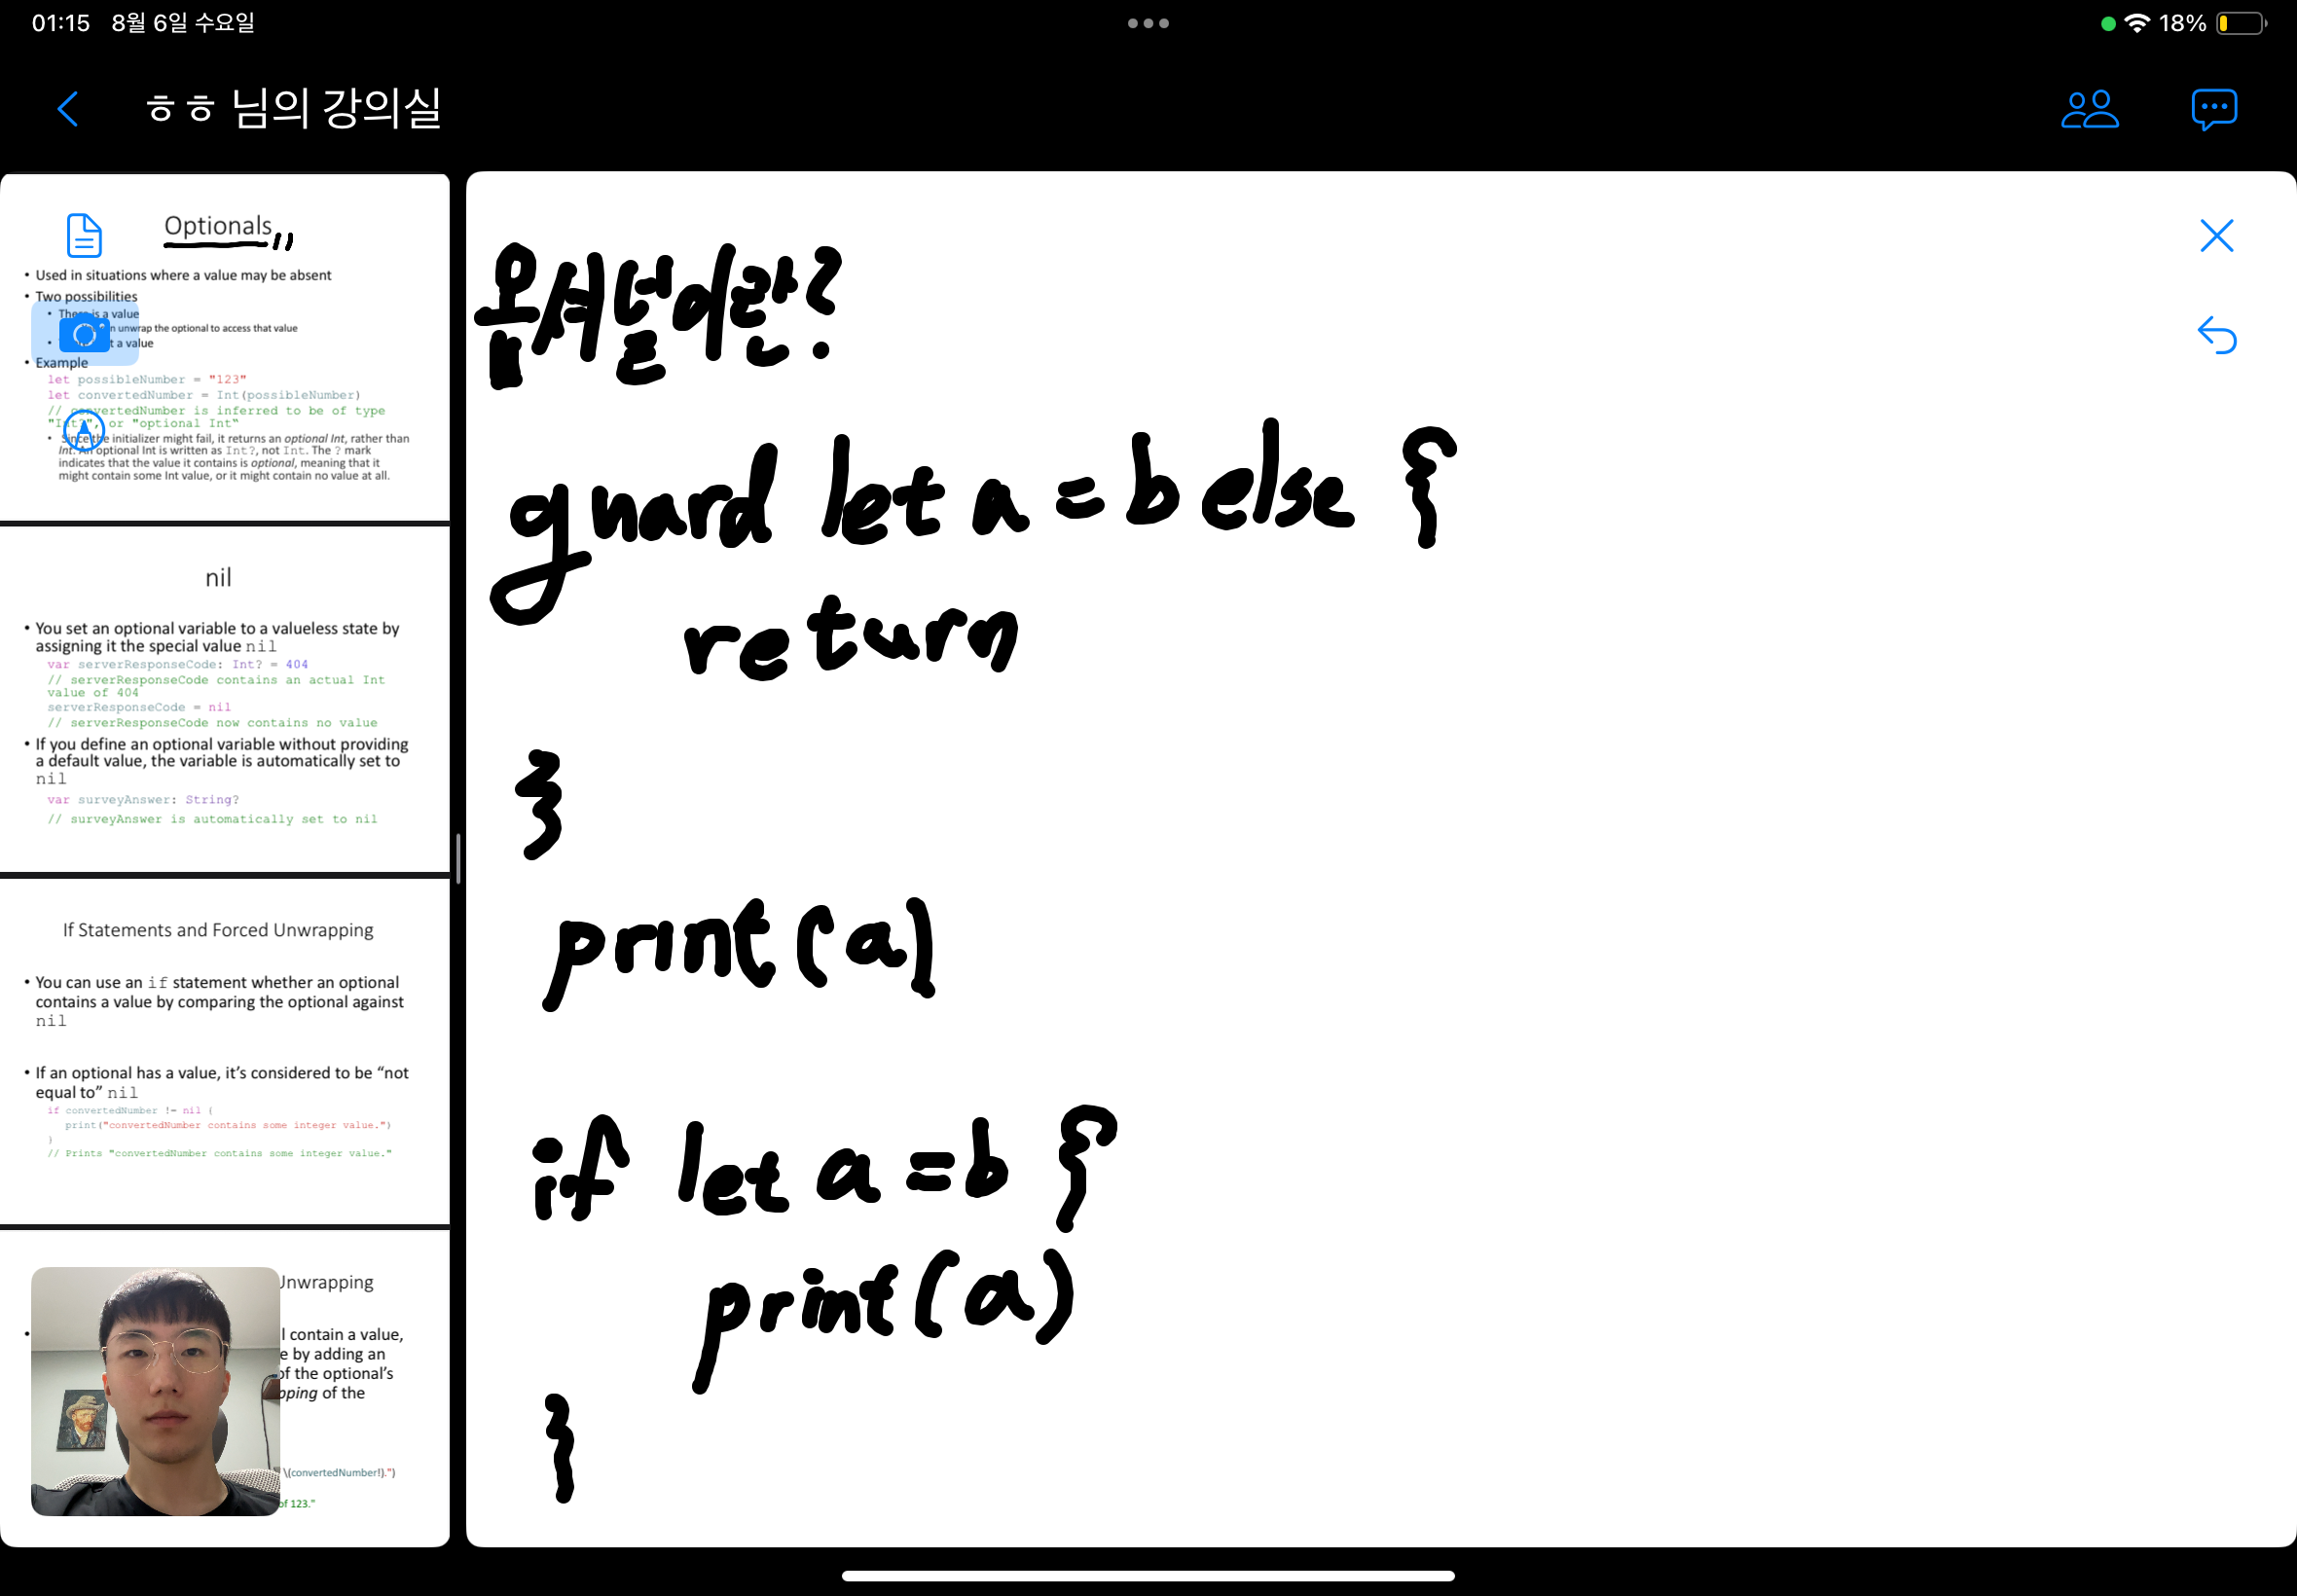
\includegraphics[width=0.9\textwidth]{UserInterfaceWithAnExpandedWhiteboardArea.PNG}
\caption{User interface with an expanded whiteboard area}\label{fig8}
\end{figure}

\noindent
grabber는 \verb+UISlider+를 기반으로 구현되었으며, 사용자의 조작으로 value가 변경되면 \verb+valueChanged+ 이벤트를 통해 강의자료와 공유 화이트보드 화면 비율을 결정하는 \verb+NSLayoutConstraint+의 \verb+multiplier+값에 해당 값을 반영하였다. \verb+UISlider+는 투명하게 설정하여 화면에 드러나지 않고 로직적인 역할만을 수행하도록 하였다.

\section{Evaluation}\label{sec4}

제시된 시스템의 학습 지원 효과와 사용 편의성을 검증하기 위해 사용자 만족도 조사를 실시하였다. 평가는 총 5명을 대상으로 진행되었으며, 비교 대상 시스템은 강의자료와 화이트보드를 함께 배치하지 않고 둘 중 하나만 표시 가능한 Cisco Webex, 강의자료와 화이트보드가 5:5로 고정된 시스템, User-Adjustable UI를 적용한 시스템 위 세 가지였다.

각 시스템을 활용하여 강의를 진행한 후, 다음 세 질문에 대한 응답을 조사하였다. 첫째, 강의자료는 학습하기에 충분히 잘 보였는가? 둘째, 그리기 기능(PDF 주석 또는 화이트보드)은 공간과 사용성 면에서 학습에 효과적으로 잘 활용되었는가? 셋째, 전체적으로 강의를 이해하기에 불편함은 없었는가? 각 항목에 대해 만족도에 따라 1점에서 5점을 평가하도록 하였으며, 그 결과는 아래의 표\ref{tab1}, \ref{tab2}, \ref{tab3}에서 확인할 수 있다.

표\ref{tab1}은 `강의자료가 학습하기에 충분히 잘 보였는가'에 대한 응답 결과다. Webex는 모든 응답자에게 최고 점수를 받아, 강의자료 단일 배치가 학습자의 가독성을 충분히 보장하였음을 확인할 수 있다. 그러나 5:5 고정 UI 시스템은 강의자료 영역이 작은 크기로 고정되어 있어 평균 2.6점으로 낮게 나타났다. User-Adjustable UI 시스템도 모든 응답자에게 최고 점수를 받았는데, 이는 상황에 따라 강의자료 영역을 확장할 수 있는 점이 학습자의 가독성을 충분히 확보할 수 있었다고 해석된다.

\begin{table}[h]
\caption{Respondents' perception of the clarity and visibility of lecture materials}\label{tab1}
\begin{tabular*}{\textwidth}{@{\extracolsep\fill}lcccccc}
\toprule%
Target System & \multicolumn{5}{@{}c@{}}{Respondents} & Average\\\cmidrule{2-6}
& 1 & 2 & 3 & 4 & 5 &\\
\midrule
Webex  & 5 & 5 & 5 & 5 & 5 & 5 \\
5:5 Fixed UI  & 1 & 5 & 1 & 2 & 4 & 2.6 \\
User-Adjustable UI  & 5 & 5 & 5 & 5 & 5 & 5 \\
\botrule
\end{tabular*}
\footnotetext{Question: Were the lecture materials clear and visible to support effective learning?}
\end{table}

\noindent
표\ref{tab2}는 `그리기 기능(PDF 주석 또는 화이트보드)은 공간과 사용성 면에서 학습에 효과적으로 잘 활용되었는가'에 대한 응답 결과다. Webex는 평균 3.8점으로, 강의자료에 주석이 가능하지만 화이트보드를 사용하기 위해서는 강의자료를 종료해야해서 강의자료와 화이트보드를 함께 활용하지 못한다는 한계가 반영된 것으로 보인다. 5:5 고정 UI 시스템은 평균 3.4점으로, 강의자료와 화이트보드를 함께 배치하긴 하지만 작은 크기로 고정되어 있어 효과적으로 활용되지 못했음을 보여준다. 반면에 User-Adjustable UI 시스템은 모든 응답자에게 최고 점수를 받았는데, 이는 강의자료를 확장하여 주석을 달거나 화이트보드를 확장하여 판서를 진행하는 등 상황에 맞는 활용이 가능했기 때문이다.

\begin{table}[h]
\caption{Respondents' perception of the usefulness and spatial sufficiency of the drawing feature (PDF annotation or whiteboard)}\label{tab2}
\begin{tabular*}{\textwidth}{@{\extracolsep\fill}lcccccc}
\toprule%
Target System & \multicolumn{5}{@{}c@{}}{Respondents} & Average\\\cmidrule{2-6}
& 1 & 2 & 3 & 4 & 5 &\\
\midrule
Webex  & 5 & 4 & 3 & 3 & 4 & 3.8 \\
5:5 Fixed UI  & 3 & 5 & 2 & 2 & 5 & 3.4 \\
User-Adjustable UI  & 5 & 5 & 5 & 5 & 5 & 5 \\
\botrule
\end{tabular*}
\footnotetext{Question: Was the drawing feature (PDF annotation or whiteboard) effectively utilized for learning in terms of space and usability?}
\end{table}

\noindent
표\ref{tab3}은 `전체적으로 강의를 이해하기에 불편함은 없었는가'에 대한 응답 결과다. Webex는 평균 4.0점으로 긍정적인 평가를 받았지만 화이트보드 활용의 한계로 인해 약간의 감점을 받았다. 5:5 고정 UI 시스템은 평균 2.4점으로 가장 낮았는데, 많은 응답자들이 작은 크기의 강의자료로 인한 학습 경험 저하를 이유로 꼽았다. 반면, User-Adjustable UI 시스템은 평균 4.6점으로 가장 높은 점수를 받았다.

\begin{table}[h]
\caption{Respondents' perception of the overall comprehensibility of a lecture}\label{tab3}
\begin{tabular*}{\textwidth}{@{\extracolsep\fill}lcccccc}
\toprule%
Target System & \multicolumn{5}{@{}c@{}}{Respondents} & Average\\\cmidrule{2-6}
& 1 & 2 & 3 & 4 & 5 &\\
\midrule
Webex  & 5 & 5 & 3 & 4 & 3 & 4 \\
5:5 Fixed UI  & 3 & 2 & 2 & 1 & 4 & 2.4 \\
User-Adjustable UI  & 4 & 4 & 5 & 5 & 5 & 4.6 \\
\botrule
\end{tabular*}
\footnotetext{Question: Was the lecture overall easy to understand?}
\end{table}

\noindent
세가지 시스템에 대한 만족도 조사 결과를 종합하면, 본 보고서에서 제시한 User-Adjustable UI 시스템은 기존 원격 교육 시스템(Webex)과 단순 병렬 제공하는 5:5 고정 UI 시스템에 비해 전반적으로 높은 사용자 만족도를 보였다. Webex는 강의자료를 크게 제공한다는 장점이 있으나 화이트보드와 동시에 활용하지 못한다는 한계가 있었고, 5:5 고정 UI 시스템은 강의자료와 화이트보드를 동시에 사용할 수 있으나 각 요소가 지나치게 작아 학습 효과가 저하되는 문제가 있었다. 반면, 본 보고서에서 제시된 User-Adjustable UI 시스템은 이 두 시스템의 상반된 한계를 보완하여 강의자료와 화이트보드를 동시에 충분한 크기로 제공할 수 있었다.

\section{Conclusion}\label{sec5}

본 보고서에서는 강의자료와 화이트보드를 동시에 시각적으로 제공하지 못하는 기존 시스템의 한계를 해결하기 위해 User-Adjustable UI 기반의 모바일 원격 교육 시스템을 설계 및 구현하였다. 제시된 시스템은 grabber를 통해 두 콘텐츠 영역의 비율을 상황에 맞게 조절할 수 있도록 하여, 제한된 크기의 모바일 기기 화면에서도 학습자가 필요한 정보를 충분한 크기로 확인할 수 있게 하였다. 또한 참여자 목록과 채팅창은 접이식 구조로 구현하여 불필요한 화면 점유를 최소화함으로써 제한된 화면 공간의 활용도를 높이고 학습 콘텐츠에 대한 시각적 집중을 강화하였다.

사용자 만족도 조사 결과, 제시된 시스템은 평가 항목인 강의자료의 가독성, 그리기 기능의 활용성, 강의 이해도 세 측면에서 모두 다른 시스템보다 우수한 평가를 받아, User-Adjustable UI가 모바일 원격 교육 환경에서 학습 효과를 향상시키는 것을 확인하였다.

전체 소스코드는 \url{https://github.com/H0sungKim/CollaborativeComputingLab}에서 확인할 수 있다.

%===========================================================================================%%
%% If you are submitting to one of the Nature Portfolio journals, using the eJP submission   %%
%% system, please include the references within the manuscript file itself. You may do this  %%
%% by copying the reference list from your .bbl file, paste it into the main manuscript .tex %%
%% file, and delete the associated \verb+\bibliography+ commands.                            %%
%%===========================================================================================%%

\bibliography{bibliography}

\end{document}
